\documentclass[
	a4paper,
	pagesize,
	pdftex,
	12pt,
	twoside, % + BCOR darunter: für doppelseitigen Druck aktivieren, sonst beide deaktivieren
	BCOR=5mm, % Dicke der Bindung berücksichtigen (Copyshop fragen, wie viel das ist)
	USenglish,
	fleqn,
	final,
	]{scrartcl}
\usepackage{ucs}
\usepackage[utf8x]{inputenc} % Eingabekodierung: UTF-8
\usepackage[T1]{fontenc} % ordentliche Trennung
\usepackage[USenglish]{babel}
\usepackage{lmodern} % ordentliche Schriften
\usepackage[unicode=true]{hyperref}
\usepackage{setspace,graphicx,tikz,tabularx} % für Elemente der Titelseite
\usepackage[draft=false,babel,tracking=true,kerning=true,spacing=true]{microtype} % optischer Randausgleich etc.
\usepackage{amsfonts}
\usepackage{enumitem}
\usepackage{algorithm}% http://ctan.org/pkg/algorithms
\usepackage{algpseudocode}% http://ctan.org/pkg/algorithmicx
\usepackage{amsthm}
\usepackage{url}
\usepackage{colortbl}
\usepackage{tabulary}
\usepackage{listings}
\usepackage{graphicx}
\usepackage{subcaption}
\usepackage{svg}

%Anpassung von Kopf- und Fußzeile
%beinflusst die erste Seite des Kapitels
\usepackage[automark,headsepline]{scrlayer-scrpage}


\ihead{\leftmark}
\chead{}
\ohead{\thepage}
\ifoot*{}
\cfoot[\thepage]{}
\cfoot*{}
\ofoot*{}
\pagestyle{scrheadings}

\algnewcommand\algorithmicforeach{\textbf{for each}}
\algdef{S}[FOR]{ForEach}[1]{\algorithmicforeach\ #1\ \algorithmicdo}
\renewcommand{\algorithmicrequire}{\textbf{Input:}}
\renewcommand{\algorithmicensure}{\textbf{Output:}}

\algdef{SE}[PROCEDURE]{Procedure}{EndProcedure}%
   [2]{\algorithmicprocedure\ \textproc{#1}\ifthenelse{\equal{#2}{}}{}{(#2)}}%
   {\algorithmicend\ \algorithmicprocedure}%
\algdef{SE}[FUNCTION]{Function}{EndFunction}%
   [2]{\algorithmicfunction\ \textproc{#1}\ifthenelse{\equal{#2}{}}{}{(#2)}}%
   {\algorithmicend\ \algorithmicfunction}%

\begin{document}

% LaTeX-Vorlage für die Titelseite und Selbständigkeitserklärung einer Abschlussarbeit
% basierend auf der vorigen Institutsvorlage des Instituts für Informatik
% sowie der Vorlage für Promotionsarbeiten.
%
% erweitert: 2014-06-12 Dennis Schneider <dschneid@informatik.hu-berlin.de>

% gepunktete Linie unter Objekt:
\newcommand{\TitelPunkte}[1]{%
  \tikz[baseline=(todotted.base)]{
    \node[inner sep=1pt,outer sep=0pt] (todotted) {#1};
    \draw[dotted] (todotted.south west) -- (todotted.south east);
  }%
}%

% gepunktete Linie mit gegebener Länge:
\newcommand{\TitelPunktLinie}[1]{\TitelPunkte{\makebox[#1][l]{}}}

\makeatletter

\newcommand*{\@titelTitel}{Titel der Arbeit}
\newcommand{\titel}[1]{\renewcommand*{\@titelTitel}{#1}} % Titel der Arbeit
\newcommand*{\@titelArbeit}{Arbeitstyp}
\newcommand{\typ}[1]{\renewcommand*{\@titelArbeit}{#1}} % Typ der Arbeit
\newcommand*{\@titelGrad}{akademischer Grad}
\newcommand{\grad}[1]{\renewcommand*{\@titelGrad}{#1}} % Akademischer Grad
\newcommand*{\@titelAutor}{Autor}
\newcommand{\autor}[1]{\renewcommand*{\@titelAutor}{#1}} % Autor der Arbeit
\newcommand*{\@titelGeburtsdatum}{\TitelPunktLinie{2cm}}
\newcommand{\gebdatum}[1]{\renewcommand*{\@titelGeburtsdatum}{#1}} % Geburtsdatum des Autors
\newcommand*{\@titelGeburtsort}{\TitelPunktLinie{5cm}}
\newcommand{\gebort}[1]{\renewcommand*{\@titelGeburtsort}{#1}} % Geburtsort des Autors
\newcommand*{\@titelGutachterA}{\TitelPunktLinie{5cm}}
\newcommand*{\@titelGutachterB}{\TitelPunktLinie{5cm}}
\newcommand{\gutachter}[2]{\renewcommand*{\@titelGutachterA}{#1}\renewcommand*{\@titelGutachterB}{#2}} % Erst- und Zweitgutachter
\newcommand*{\@titelEinreichungsdatum}{\TitelPunktLinie{3cm}} % Datum der Einreichung, wird nicht vom Studenten ausgefüllt
\newcommand*{\@titelVerteidigungsdatum}{} % Verteidigungstext, wird nicht vom Studenten ausgefüllt
\newcommand{\mitverteidigung}{\renewcommand*{\@titelVerteidigungsdatum}{verteidigt am: \,\,\TitelPunktLinie{3cm}}} % Verteidigungsplatzhalter erzeugen
\newcommand*{\@wastwoside}{}

% Titelseite erzeugen:
\newcommand{\makeTitel}{%
	% Speichere, ob doppelseitiges Layout gewählt wurde:
\if@twoside%
	\renewcommand*{\@wastwoside}{twoside}
\else
	\renewcommand*{\@wastwoside}{twoside=false}
\fi
	\KOMAoptions{twoside = false}% Erzwinge einseitiges Layout (erzeugt eine Warnung)

	\begin{titlepage}
		% Ändern der Einrückungen
		\newlength{\parindentbak} \setlength{\parindentbak}{\parindent}
		\newlength{\parskipbak} \setlength{\parskipbak}{\parskip}
		\setlength{\parindent}{0pt}
		\setlength{\parskip}{\baselineskip}

		\thispagestyle{empty}

		\begin{minipage}[c][3cm][c]{12cm}
			\textsc{%
				% optischer Randausgleich per Hand:
				\hspace{-0.4mm}\textls*[68]{\Large Humboldt-Universität zu Berlin}\\
				\normalsize \textls*[45]{
					Mathematisch-Naturwissenschaftliche Fakultät\\
					Institut für Informatik
				}
			}
		\end{minipage}
		\hfill


		% Also wenn schon serifenlose Schriften (Titel), dann ganz oder gar nicht
		\sffamily

		\vfill

		\begin{center}
		\begin{doublespace}
			\vspace{\baselineskip}
			{\LARGE \textbf{\@titelTitel}}\\
			%\vspace{1\baselineskip}
			{\Large
				\@titelArbeit\\
				zur Erlangung des akademischen Grades\\
				\@titelGrad
				\vspace{\baselineskip}
			}
		\end{doublespace}
		\end{center}

		\vfill
\newcolumntype{L}{>{\raggedright\arraybackslash}X}
		{\large \raggedleft
			\begin{tabularx}{\textwidth}{l@{\,\,\raggedright~}L} % verbreiterter Abstand zwischen Feldern wurde gewünscht
				eingereicht von: & \@titelAutor\\
				geboren am: & {\@titelGeburtsdatum}\\
				geboren in: & \@titelGeburtsort
				\vspace{0.5\baselineskip}\\
				Gutachter/innen: & \@titelGutachterA \\
					& \@titelGutachterB
				\vspace{0.5\baselineskip}\\
				eingereicht am: & \@titelEinreichungsdatum \hfill \@titelVerteidigungsdatum
			\end{tabularx}}
			\vspace{-1\baselineskip}\\\phantom{x} % Übler Hack, um eine Warnung wg. einer zu leeren hbox zu verhindern
		% Wiederherstellen der Einrückung
		\setlength{\parindent}{\parindentbak}
		\setlength{\parskip}{\parskipbak}
	\end{titlepage}

	% Aufräumen:
	\let\@titelTitel\undefined
	\let\titel\undefined
	\let\@titelArbeit\undefined
	\let\typ\undefined
	\let\@titelGrad\undefined
	\let\grad\undefined
	\let\@titelAutor\undefined
	\let\autor\undefined
	\let\@titelGeburtsdatum\undefined
	\let\gebdatum\undefined
	\let\@titelGeburtsort\undefined
	\let\gebort\undefined
	\let\@titelGutachterA\undefined
	\let\@titelGutachterB\undefined
	\let\gutachter\undefined
	\let\@titelEinreichungsdatum\undefined
	\let\einreichungsdatum\undefined
	\let\@titelVerteidigungsdatum\undefined
	\let\verteidigungsdatum\undefined
	\let\@titelBetreuer\undefined
	\let\betreuer\undefined

	\KOMAoptions{\@wastwoside}% Stelle alten Modus (ein-/doppelseitig) wieder her
	\let\@wastwoside\undefined
	\cleardoublepage % ganzes Blatt für die Titelseite
}

% Als Allerallerletztes kommt Selbständigkeitserklärung:
% Aufruf mit dem Datum in deutscher und englischer Form
\newcommand{\selbstaendigkeitserklaerung}[1]{%
	\cleardoublepage% Wieder auf eine eigene Doppelseite
	\thispagestyle{plain}

	{\parindent0cm
		\subsection*{Selbständigkeitserklärung}
		Ich erkläre hiermit, dass ich die vorliegende Arbeit selbständig verfasst
		und noch nicht für andere Prüfungen eingereicht habe.
		Sämtliche Quellen einschließlich Internetquellen, die unverändert oder
		abgewandelt wiedergegeben werden, insbesondere Quellen für Texte, Grafiken,
		Tabellen und Bilder, sind als solche kenntlich gemacht. Mir ist bekannt,
		dass bei Verstößen gegen diese Grundsätze ein Verfahren wegen
		Täuschungsversuchs bzw. Täuschung eingeleitet wird.
		\vspace{3\baselineskip}

		{\raggedright Berlin, den #1 \hfill \TitelPunktLinie{8cm}\\}
%		\vspace{3\baselineskip}
%
% 		\selectlanguage{english}
% 		\subsection*{Statement of authorship}
% 		Hier würde die englische Selbständigkeitserklärung folgen, falls gewünscht. Doch es fehlt eine akzeptable Übersetzung.
% 		\vspace{3\baselineskip}
%
% 		Berlin, #2 \hfill \TitelPunktLinie{6cm}
	}
}%

\makeatother

\titel{Practical Applications of One-to-Many Matchings with One-Sided Preferences} % Titel der Arbeit
\typ{Bachelorarbeit} % Typ der Arbeit:  Diplomarbeit, Masterarbeit, Bachelorarbeit
\grad{Bachelor of Science (B. Sc.)} % erreichter Akademischer Grad
\autor{Aaron Oertel} % Autor der Arbeit, mit Vor- und Nachname
\gebdatum{18.02.1997} % Geburtsdatum des Autors
\gebort{Dinslaken} % Geburtsort des Autors
\gutachter{Prof. Dr. Henning Meyerhenke}{Prof. Dr. Timo Kehrer}
\mitverteidigung % entfernen, falls keine Verteidigung erfolgt

\pagenumbering{alph}
\makeTitel

\pagenumbering{Roman}
\section*{Abstract}\label{sec:abstract}

Matching algorithms are of great interest due to the diverse use cases that exist in the real world. This thesis explores matching mechanisms for one-to-many matching scenarios with one-sided preferences by using the student-seminar assignment problem as a motivating example. We first discuss several optimality criteria and four algorithms with different characteristics before investigating the algorithms' performance characteristics in theoretical and experimental settings. The experiments show that reducing the problem to the assignment problem or performing a min-weight max-cardinality matching on the problem's induced bipartite graph yields the best results for most metrics and instances. Additionally, an interactive web system is presented that allows for managing and solving such matching problems by employing the presented algorithms. 

\newpage
\tableofcontents

\newpage
\listoffigures
 
\newpage
\listoftables

\newpage
\pagenumbering{arabic}
\section{Introduction}
\label{sec:introduction}

\subsection{Motivation}
Many institutions around the world use central, automated matching schemes to assign agents to resources, based on their preferences. For instance, the National Resident Matching Program (NRMP) in the United States uses such a matching mechanism to pair graduating medical students to residency positions at hospitals every year \cite{Roth-NRMP}. There are different goals for these matchings, which can range from efficiency to fairness, and finding a mechanism that fulfills these goals is an important task to efficiently design such markets.
There are also many variants of matching problems, that include but are not limited to one-to-one, one-to-many and many-to-many matchings. The distribution of preferences need to be considered as well. For instance, in the hospital-residents problem, both the hospitals and residents supply preferences over the other set. Here it is important to consider if incomplete preference lists or ties should be allowed in the matchings. 

This thesis will formally describe, examine and analyze the problem of one-to-many matching mechanisms with one-sided preferences. While there are many use-cases for this problem, we will focus on the problem of matching students to seminars, which is of high interest for many universities, who often require their students to participate in a seminar in order to obtain their degree. These students typically have a choice between a handful of different seminars; however, there are capacity constraints that make it hard to match all students to their first choice. Let us consider the following example: 100 students have to be assigned to one of six seminars, wherein each seminar has a capacity of 20 students. The students express their preferences by supplying a strict, meaning without ties, but possibly incomplete preference list of the six seminars. The goal for the school's administration now is to find an assignment of students to seminars that fulfills their requirements, which can range from assigning as many students as possible to being as fair as possible with the assignments. We will see that there is no obvious choice in picking an algorithm, since there are plenty of trade-offs between existing mechanisms that make it necessary to prioritize the requirements.  
What makes this problem harder is that the students' preferences are not necessarily equally distributed. Oftentimes a majority of students prefer one seminar which conflicts with other students getting their first choice. At the same time, it can occur that students go unmatched when their preference lists are short and primarily consist of seminars that have already reached full capacity.

The goal of this thesis is to formally model the one-to-many matching problem with one-sided preferences, while presenting different algorithms for finding matchings and finally to evaluate these algorithms using certain metrics that make sense in the one-to-many case. For the purpose of this thesis, we will use the example of student-seminar matching to analyze the problem, but it is important to note that it can just as well be generalized to any other one-to-many matching problem with incomplete preferences. Lastly, an interactive system will be developed, which will allow a school's administration to find a student-seminar matching using one of the presented algorithms. 

\subsection{Formal Definition}
The problem of assigning students to seminars can be described as a many-to-one matching, with a set of students $S:= \{s_1, s_2, ...,s_n\}$ and a set of seminars $T:= \{t_1, t_2, ..., t_m\}$. Every student $s_i \in S$ provides a strict, i.e. tie-less, preference order over a subset of $T$, and every seminar $t_j \in T$ has a capacity of $c_j$ students. The goal is to find a matching $M: S \rightarrow T$, that assigns students to one of their preferred seminars while respecting the capacity of the seminars. That means that for every seminar $t_j$ the following is satisfied: $|M^{-1}(t_j)| \leq c_j$. Using this definition we can describe the problem as a many-to-one matching with one-sided, incomplete preferences. In the case of students and seminars this means that one student is matched to one seminar, but one seminar is matched to a number of students, while only students express their preferences over the seminars. Later, we will discuss different optimality criteria, which can be used for defining an objective function for the problem.

\subsection{The Capacitated House Allocation Problem}\label{intro:cha}
Many economists and game theorists \cite{FEKETE2003219} have studied variants of the house allocation (HA) problem, wherein a set of indivisible items $H$, the houses, needs to be divided among a set $A$ of applicants. Each applicant may have a strict preference order over a subset of $H$. Formally this means that an instance $I$ of the problem consists of two disjoint sets, where $H := \{h_1, h_2, ..., h_n\}$ is the set of houses and $A := \{a_1, a_2, ..., a_m\}$ is the set of applicants. Each applicant $a_i \in A$ ranks a subset of the houses in $H$ using a preference list. The houses, on the other hand, do not have any preferences over applicants. A matching or assignment $M$ is map with $M: A \rightarrow H$, so that for every applicant $a_i$, the house $M(a_i)$ is on the applicants preference list \cite{SngThesis}. 

The house allocation problem is essentially an alias for a matching problem on bipartite graphs with one-sided preferences. There are many applications including matching clients to servers, professors to offices and also students to seminars. For the latter, some generalizations have to be made to the problem; specifically, one seminar should now be matched to more than one student, whereas the houses in HA are matched to one and only one applicant. In the literature, the latter variant of the problem is also referred to as the "Capacitated House Allocation Problem", denoted by CHA \cite{algorithmics}. The following chapters of this thesis will explore performance indicators and algorithms for finding matchings in the context of students and seminars, which is semantically equivalent to the CHA problem.

\subsection{Outline}
Given this problem definition, we will review the literature for optimality criteria and, based on that criteria, present algorithms that produce matchings with those characteristics. Many of those charactistics are quite obvious such as maximum-cardinality; however, we will also review terms such as "Pareto-efficiency" or "Popularity" that are commonly used in the context of market design and game theory. 
Using these criteria, we will review matching algorithms that solve the problem and then analyze and compare their runtime-complexity and optimality-properties. We will see that no algorithm is known that fulfills all desirable properties, which makes it necessary to understand the trade-offs and relationships between the algorithms. 

After completing a theoretical comparison of the algorithms, we will proceed to analyze matchings computed using real data to better understand the theoretical observations and trade-offs discussed before. Additionally, a web-interface will be presented that allows a university's administration to compute matchings according to their requirements using data that the system receives as input. Lastly, we will briefly explore extensions to the problem, such as the many-to-many case and finally summarize the result and make recommendations for the implementation and usage of the system, based on the current state of research on these matching mechanisms.

Therefore, the contribution of this thesis is a practically motivated survey and analysis of one-to-many matchings with one-sided preferences. We use the problem of matching students to seminars as a motivating example to understand commonly used algorithms and their performance characteristics, by performing both a theoretical and a practical analysis using real and synthesized data. This will conclude with recommendations for building such systems, based on the theoretical and practical results obtained in the previous sections. 

\subsection{Related Problems}
There are many related matching problems that can be classified as follows:
\begin{enumerate}
    \item Bipartite matching problems
    \begin{enumerate}
        \item One-sided preferences \ref{intro:cha}
        \begin{enumerate}
            \item One-to-one (e.g. House Allocation problem)
            \item \textbf{One-to-many (e.g. Capacitated House Allocation problem)} 
        \end{enumerate}
        \item Two-sided preferences
        \begin{enumerate}
            \item One-to-one (e.g. Stable-Marriage problem) \ref{intro:stable-marriage}
            \item One-to-many (e.g. Hospital-Residents problem) \ref{intro:hospital-residents}, \ref{extensions:two-sided}
        \end{enumerate}
    \end{enumerate}
    \item Non-bipartite matching problems 
    \begin{enumerate}
        \item One-to-one (e.g. Stable-Roommates problem)
    \end{enumerate}
\end{enumerate}
Even though these problems have some differences, key mechanisms (section \ref{chapter:algorithms}) and optimality criteria (section \ref{sec:optimality}) used for them can nonetheless be similar or even identical. For instance, in the case of one-sided preferences, mechanisms for the one-to-one case can often easily be extended to the one-to-many case. It is also important to note that the problem can be extended to using incomplete preference lists and ties in the preference lists. In fact, real-world settings often necessitate at least incomplete preference lists, as students often want to classify a seminar as unacceptable. The following subsections will briefly present some of the listed matching problems and present their key results.  

\subsubsection{Stable Marriage Problem}\label{intro:stable-marriage}
The stable marriage problem was one of the first matching problems to be researched \cite{GaleShapleyOrig}, and consequently motivated further research in the field of matching under preferences.

The problem is stated as follows: A set of men $M$ and of women $W$ shall be matched one-to-one, where each men and women provide a complete strict-preference order over the agents of the other set. The deferred acceptance algorithm presented in Gale and Shapley's paper \cite{GaleShapleyOrig} finds a \emph{stable}, complete matching in polynomial time. Stability is defined as follows: given a women $w \in W$ and any man $m \in M$ that she was not matched to, $w$ does not prefer $m$ more than her current partner, and $m$ does not prefer $w$ more than his current partner. Therefore, in a stable matching, no pair of applicants $(m, w)$ should exist, so that $m$ and $w$ would benefit from leaving their assigned partner to be with each other.

The deferred acceptance algorithm uses one of the sets of applicants, for example the men, and proceeds by letting every man propose to their most preferred woman. The woman will tentatively accept the proposal, if she is not engaged at that point, or prefers the new proposal over her previous one. Then the algorithm repeats this process with men proposing to their most-preferred, but not yet proposed to woman until they are either matched or have no more women to propose to \cite{Gusfield}.

It is important to note that the algorithm produces different results if the women are the proposers: It has been shown that all possible executions of the algorithm with men as proposers yield the same stable matching. That matching is men-optimal, which means that every man has the best partner that he can have in any stable matching \cite{Gusfield}. Additionally, with men proposing, the produced matchings have also been shown to be women-pessimal, meaning that every woman is matched to the worst partner that she can have in any matching \cite{Gusfield}.

While the scenario of matching women to men like described is presumably not a common real-world occurrence, Gale and Shapley's paper inspired several new approaches to other similar problems.

\subsubsection{Hospitals/Residents Problem}\label{intro:hospital-residents}
A few years after the publication of Gale and Shapley's original paper, it was determined that the deferred acceptance mechanism was essentially the same mechanism used by the National Resident Matching Program (NRMP) in the United States to match graduating medical students to residency positions in hospitals \cite{Gusfield}. As a matter of fact, Gale and Shapley's paper described an algorithm for the so-called "college admissions problem"\cite{GaleShapleyOrig}, which is essentially the same problem. Just like in the stable-marriage problem, there is a solution that can be hospital-optimal or resident-pessimal. 

The problem can be described as finding a one-to-many matching with two-sided, incomplete, but strict preferences. Essentially, a hospital can offer multiple spots and both parties can mark entities from the other set as unacceptable by not including them in their preference lists \cite{RePEc:ris:nobelp:2012_005}. Therefore the main difference to the stable marriage problem is that one and only one of the sets allows their entities to have a capacity, i.e. accept more than one applicant. At the same time though, entities in both sets still express preferences, which makes this problem different from the CHA-problem \ref{intro:cha} where only entities from one set express preferences.

In reality, the problem solved by the NRMP is more complex, as it permits couples of residents to submit preferences together. It has been shown that a stable solution does not always exist and that finding one if it exists, or showing that it doesn't exist is NP-complete \cite{RONN1990285}. The revised algorithm used by the NRMP utilizes findings about stability and simple matching markets to find a good approximation, while minimizing opportunities for strategic manipulation, which was indeed possible before \cite{NBERw6963}.

\subsubsection{Assignment Problem}\label{intro_assignment}
The problem of matching students to seminars can also be defined as an assignment problem. The goal of the assignment problem is to find a minimum-weight, perfect matching in a bipartite graph. In this case the goal of the problem is, given the set of students $S$, seminars $T$, and a cost function $W: S \times T \rightarrow \mathbb{R}$, to find a map $M: S \rightarrow T$, which minimzes the following objective function:
$\sum_{s \in S} W(s, M(s))$.

One of the first algorithms used for solving this problem was the Hungarian algorithm by Munkres, which finds a minimum-weight matching in polynomial time \cite{Munkres}. 
Alternatively, the problem can be transformed into an instance of the minimum-cost flow problem to determine a minimum weight matching. Section \ref{algo:assignment} will further investigate using this algorithm for the problem of student-seminar matching.

\subsubsection{The Student-Project Allocation Problem}
A similar problem to the CHA or student-seminar assignment problem is the Student-Project Allocation problem (SPA). This problem considers three entities instead of two, which are students, projects and lecturers. In most variations of the problem, students have preferences over courses, while courses again have capacities. However, lecturers are also considered, where lecturers can have preferences over students and/or courses. Algorithmic approaches used for this problem are mostly based on the deferred acceptance mechanism and find stable matchings that can either favor the students or lecturers \cite{algorithmics}. 

\newpage
\section{Optimality criteria}
Looking at the previously presented problems, it is clear that there are different objective functions or optimality criteria for such matchings. For instance, in the stable marriage problem, matchings are primarily judged by the stability characteristic. However such a characteristic does not make sense in the case of the student-seminar problem, since stability assumes both-sided preferences. For that very reason, different criteria have to be used for judging the quality of a matching.
\newline
Intuitively, when thinking about matching students to seminars, it would be desirable to match as many students as possible, as well as matching the students to their first choice, but at the same time to be fair and resistant to manipulation. To formalize these requirements, a few criteria have been discussed in the literature, which will be helpful for comparing different approaches. 

\subsection{Maximum cardinality}
The goal of the maximum cardinality problem is finding a matching $M$ on a graph $G=(V=(X, Y), E)$, so that $|M|$ is maximal.\cite{GraphTheoryIntro} Consequently, maximum cardinality as an optimality criteria means that a matching is ideal if the number of students that are matched is maximized among all possible matchings. It should be noted here, that the student's preferences are not considered when computing the maximum cardinality matching. As a matter of fact, it is possible that multiple matchings of the same cardinality exist, where one of the matchings could be better in the sense of a different optimality criteria. Therefore, maximum cardinality may be desirable, but should be used in conjunction with a different criteria, as it does not consider student preferences. This criteria is also often referred to as efficiency in the literature, however we will use the term maximum-cardinality as it is more specific.

\subsection{Pareto-Optimality}
Pareto optimality or Pareto efficiency is a commonly used term in economics to describe the state of resource allocations. Intuitively an allocation, or in our case a matching, is Pareto optimal, iff no improvement can be made to a single individual, without worsening the situation for other individuals. Additionally a matching, in which two students $s_1, s_2$ would be better off by swapping their seminars is not Pareto optimal.
In order to more formally define Pareto-optimality we must first define student preferences more formally: 
\newline
Given two matchings $M, M'$ and a student $s \in S$, the student $s$ prefers $M'$ over $M$ in the following cases:
\begin{enumerate}
    \item s is matched in $M'$ and unmatched in $M$, or
    \item s is matched in both $M'$ and $M$, however prefers $M'(a)$ over $M(a)$
\end{enumerate}
Using this defintion we now define Pareto optimality as follows: Given an instance $I$ of a matching problem and its set of possible matchings $\mathcal{M}$, we define a relation $\succ$ on $\mathcal{M}$, where given two matchings $M, M' \in \mathcal{M}$ the following holds true: $M' \succ M$ if no students prefers $M$ to $M'$, but some student prefers $M'$ over $M$. Consequently a matching $M' \in \mathcal{M}$ is called Pareto-optimal iff there exists no other matching $M \in \mathcal{M}$, such that $M' \succ M$.\cite{algorithmics}
A Pareto-optimal matching always exists for any instance of a matching problem and can be efficiently computed using one of various algorithms. A simple greedy algorithm uses the random serial-dictatorship mechanism to draw each agent in random order and let's them select their most-preferred, available item from their preference list.\cite{RothTwoSided, SerialDictatorship} However the greedy algorithm does not always compute a Pareto optimal matching of maximum cardinality, which would be desirable in student-seminar matching.\cite{Abraham:Pacha}

\subsection{Popularity}
In the context of matching with one-sided preference lists, using an optimality criteria like Stability, which is based on the preferences of both parties, doesn't apply. Instead a commonly used criteria is a matching $M$'s Popularity, which indicates that more students prefer that matching $M$ over any other possible matching.\cite{ManlovePopularMatchings} Given the definition of the student-seminar matching problem, we can formally define Popularity as follows:
Let $P(M', M)$ be the set of students who prefer $M'$ over $M$. A matching $M'$ is said to be more popular than $M$, denoted by $M' \succ M$, iff $|P(M', M)| > |P(M, M')|$. That concludes that a matching $M'$ is popular, iff there is no other matching $M$ that is more popular than $M'$, i.e. $M' \succ M$.\cite{Klaus, AbrahamPopular} Due to that definition, this criteria is often also referred to as the majority assignment.\cite{Gardenfors}
\newline
Using this definition, we can see that every popular matching also is a pareto-optimal matching. Given a popular matching $M'$ and any matching $M$ for an instance $I$ of the problem, $M'$ is pareto-optimal if $P(M, M') = 0$ and $P(M', M) \geq 1$, which obviously implies that $M'$ is popular as well.\cite{Klaus}
\newline
It is important to note that a popular matching's cardinality could be smaller than the maximum cardinality, meaning that in the case of student-seminar matchings, a group of students could be left unassigned in favor of the majority of the students having a match that they prefer.
Additionally, a popular matching, unlike a pareto-optimal matching, does not always exist. To illustrate this, let's consider the following instance: $S=\{s_1, s_2, s_3\}$, $T=\{t_1, t_2, t_3\}$, where each student has the same preference list, being $t_1 < t_2 < t_3$, and each seminar $t_i \in T$ has a capacity of 1. Given the following matchings, we can confirm that there exists no popular matching for the given instance: 
\begin{enumerate}
    \item $M_1=\{(s_1, t_1), (s_2, t_2), (s_3, t_3)\}$
    \item $M_2=\{(s_1, t_3), (s_2, t_1), (s_3, t_2)\}$
    \item $M_3=\{(s_1, t_2), (s_2, t_3), (s_3, t_1)\}$
\end{enumerate}
Obviously $M_2$ is more popular than $M_1$, $M_3$ is more popular than $M_2$ and $M_1$ is more popular than $M_3$.\cite{AbrahamPopular}

\subsection{Profile-based optimality}
Contrary to Popularity and Pareto optimality, where the students' satisfaction with a matching is compared, we could also examine the structure of a matching by defining the profile of a matching and comparing it. Intuitively the profile of a matching $M$ is a vector whose $i$th component indicates the number of students obtaining their $i$th-choice seminar in $M$ according to their preference list. 
\newline
Formally, let $I$ be an instance and $\mathcal{M}$ the set of its matchings. Given a matching $M \in \mathcal{M}$ with the set of students $S$ and seminars $T$, we define the regret $r(M)$ of $M$ as follows:
$r(M) = \max \{rank(s_i, t_j): (s_i, t_j)\in M\, s_i \in S, t_j \in T\}$, where for every match $(s_i, t_j) \in M$, $rank(s_i, t_j)$ is defined as the position of $t_j$ on $s_i$'s preference list. The profile of $M$ is now defined as a vector $\langle p_1,..., p_r* \rangle$, with $r^* = r(M)$ and for each $k \in [1,r^*]$, the $k$th component is defined as: $p_k=|\{(s_i, t_j) \in M: rank(s_i, t_j) = k\}|$.\cite{algorithmics}
\newline
Using the defintion of a matching's profile, it is now possible to define a matching as rank-maximal as follows: A matching $M$ is rank-maximal, if its profile $p(M)$ is lexicographically maximum over all possible matchings in $\mathcal{M}$. That means that the number of students in $M$ who are matched to their first choice is maximum among all $M' \in \mathcal{M}$ and taking that into consideration, the number of students who are matched to their 2nd choice is maximum among all matchings, and so on.
TODO: greedy rank maximal as well? 

\subsection{Strategy-Proofness}
The previously mentioned criteria all have in common that they primarily consider the structure of a matching to evaluate quality and not the properties of a matching mechanism, i.e. algorithm. An important question to consider though, is if the agents can manipulate the outcome of an algorithm by not truthfully disclosing their preferences. Indeed, in the setting of matching residents to hospitals in the US, a previously used algorithm allowed students to improve their outcome of the algorithm by not supplying their real preferences.\cite{Gusfield} In the literature, the term for a mechanism, where no agent can benefit from misrepresenting their preferences is called strategy-proof. \cite{Klaus} Such mechanisms are of high interest for most matching problems, since preference-based optimality criteria, like the ones previously mentioned, would certainly lose some significance if the mechanism used to compute them is not strategy-proof.
For instance, it has been shown \cite{ROTH1982127}, that for the stable marriage problem with incomplete preferences, there exists no matching mechanism that both produces a popular matching and is strategy-proof.
To formalize this, we will use a game-theory definition of strategy-proofness, which goes as follows: It is a weakly dominant strategy for each agent to report their true preference list. \cite{Klaus}

\subsection{Application to student-seminar matching}\label{criteria-application}
Given the problem description of student-seminar matching, it would be desirable to find a matching that has the following properties:
\begin{enumerate}
    \item \textbf{Maximum Cardinality:} As few students as possible should be left unmatched.
    \item \textbf{Pareto Optimality:} A set of students should not feel the need to swap their match to improve their situation.
    \item \textbf{Popularity:} The number of students who are satisfied with their matching should be maximum among all possible matchings.
    \item \textbf{Rank Maximality:} As many students as possible should be matched to their first choice or if not possible second choice, and so on.
    \item \textbf{Stratey-proofness:} Students should not be able to benefit, i.e. increase their chances of being matched to their top-preference, by lying about their true-preferences. A matching mechansim should also not encourage students to supply short preference lists.
\end{enumerate}
Using these requirements, the next sections will present algorithms, for finding matchings that have some of those properties. One of these will be implemented to be used by the interactive system to find matchings which will try to optimize some of the mentioned metrics. As we have already seen, there does not always exists a popular matching or a pareto-optimal matching that is also agent complete. Additionally, the fact that students can supply incomplete preference lists, can very well lead to matchings that leave a few students unassigned, even if the sum of the capacity of all seminars is greater than the number of students. Given these constraints and observations, we will see that there is no such thing as an ideal matching for all instances based on the criteria we have presented. However, it will be possible to find matchings that will leave a majority of the students satisfied.

\newpage
\section{Algorithmic Approaches}\label{chapter:algorithms}
In the previous section, we discussed several optimality criteria that apply to the problem of matching students to seminars. This chapter will present algorithms for computing matchings that fulfill some of those criteria, as well as evaluating them against each other. The goal of this evaluation is choosing the "ideal" algorithm for implementation. We will see that each of the algorithms has some draw-backs, which might make them undesirable for the student-seminar problem. 

\subsection{Greedy with serial dictatorship}\label{algo-rsd}
One of the simplest algorithms for the student-seminar matching problem is a greedy approach, that iterates over the set of students and assigns each of the students to their most preferred seminar that still has some capacity left. In contrast to Gale \& Shapley's deferred acceptance algorithm for the stable marriage problem, this algorithm does not tentatively match students once they make their selection, but makes a final assignment for those students. Because of this, the algorithm finds a matching in $\mathcal{O}(n)$ time with $n$ being the number of students. This mechanism of letting students successively pick their highest available preference in order is known as serial dictatorship.\cite{MANEA2007316} In detail the algorithm is as follows: 

\begin{algorithm} % enter the algorithm environment
    \caption{Greedy serial dictatorship matching} 
    \label{alg1} % and a label for \ref{} commands later in the document
    \begin{algorithmic} % enter the algorithmic environment
        \Require set of Students with preferences $S$, set of Seminars $T$
        \Ensure Pareto-Optimal Matching M
        \Function{SD-Matching}{$S, T$}
        \State $M = \emptyset$
        \ForEach {$s \in \mathcal S $}
            \State $t =$ highest ranked, available seminar on preference list of s
            \If{$t \neq null$}
                \State $M = M \cup \{(s, t)\}$
            \EndIf
        \EndFor
        \State\Return M
        \EndFunction
    \end{algorithmic}
\end{algorithm}

Even though this algorithm is very simple and fast, it has some desirable properties, including one of the optimality criteria defined before:

\subsubsection{Properties}
Since the order, in which the students get to pick their match is pre-defined, we can easily show that the algorithm always produces a pareto-optimal matching.
\newtheorem{theorem}{Theorem}
\begin{theorem}
    A greedy algorithm that uses serial dictatorship always produces a pareto-optimal matching.
\end{theorem}
\begin{proof}
    Let $M$ be the matching produced by the algorithm. We assume that there exists a matching $N$ that pareto-dominates $M$. Now, let $s\in S$ be the first student who prefers his match in $N$ over $M$. Since $s$ prefers $N(s)$ over $M(s)$, the seminar $N(s)$ must have been unavailable when he made his pick. That means that another student $s' \in S$ exists, who picked $N(s)$ before $s$ could. However, we required that $s$ was matched to a better seminar in $N$, which means that $s'$ gets a worse match in $N$. This is a contradiction, so $N$ cannot pareto-dominate $M$.
\end{proof}

We can also easily see that the algorithm is strategy-proof, because every applicant makes his final pick once it's his turn, there is no benefit in misrepresenting preferences.\cite{Klaus}

\subsubsection{Drawbacks}
When looking at the algorithm, it is clear that it has a strict preference order over students, specified by the order in which students are matched in the for-loop. Additionally, the algorithm makes no effort to match all students: if it's a student's turn to pick his match, and none of the seminars on his preference lists are free, that student will not be matched at all. This problem gets worse when we consider that our problem statement allows for incomplete preference lists, which increases the chances of having a high number of unmatched students. To illustrate this let us consider the following example in Table \ref{table:1}:
\begin{table}[h!]
    \centering 
    \begin{tabular}{llll}
    Agent   & Pref list     & Seminar   & Capacity \\
    $s_1$   & $t_1$, $t_2$  & $t_1$     & 1        \\
    $s_2$   & $t_1$         & $t_2$     & 1       
    \end{tabular}
    \caption{Instance where Serial Dictatorship admits no max cardinality matching}
    \label{table:1}
\end{table} 
In this example, each seminar only has a capacity of 1 and both students have seminar $t_1$ as their first preference. If the algorithm first gives $s_1$ a chance to pick, and then $s_2$, $s_1$ will be matched to $t_1$, making $t_1$ full and not allowing $s_2$ to be matched. On the other hand, matching $s_2$ to $t_1$ first and then matching $s_1$ to $t_1$ also yields a pareto optimal matching, however, in this case, all the students are matched.

To address the other problem of preference over students, a simple approach is using the random serial dictatorship mechanism, which instead creates a random order of students as the pick order. This approach is still not fair in the sense that the first student in that order has a better chance at receiving his top priority seminar compared to all other students; however, any student has the chance to be the first one to make a pick. 

\subsection{Pareto Optimal Maximal Matchings for CHA}\label{algo-max-po}
We have seen that serial dictatorship is an easy and time-efficient mechanism for computing Pareto-optimal matchings. A big weakness of the approach, however, is that it finds just one of many possible Pareto-optimal matchings without making any guarantees about quality in regards to cardinality. Particularly, the example in Table \ref{table:1} shows how permutations of the same instance can produce matchings of different cardinality, which motivates the search for an algorithm that produces a Pareto-Optimal matching of maximum cardinality. 

(TODO: cited) Abraham et. al \cite{Abraham:Pacha} have proposed a 3-phase algorithm for computing a maximum cardinality matching for the house allocation problem, which was extended by Sng \cite{SngThesis} for the many-to-one case. Before presenting the algorithm, an important lemma about Pareto optimal matchings has to be shown first, which is then used for proofing the correctness of the algorithm. To characterize the lemma, we need to define the terms maximality, trade-in-free and cyclic coalition in regards to a matching $M$ first: 
\begin{enumerate}
    \item \textbf{Maximal}: $M$ is maximal, if no student $s_i \in S$ and seminar $t_j \in T$ exists, so that $s_i$ is unassigned, $t_j$ is undersubscribed in $M$ and $t_j$ is on $s_i$'s preference list.\cite{Abraham:Pacha}
    \item \textbf{Trade-in-free}: $M$ is trade-in-free, if there are no student $s_i \in S$ and seminars $t_j, t_l \in T$, such that $s_i$ is assigned to $t_l$, but prefers $t_j$ over $t_l$ and $t_j$ is undersubscribed.\cite{Abraham:Pacha} 
    \item \textbf{Cyclic coalition}: $M$ contains a cyclic coalition, if there exists a sequence of distinct assigned students $C = \langle s_0, s_1, \dots, s_{r-1} \rangle$ with $r \geq 2$, such that $s_i$ prefers $M(s_{i + 1 \bmod r})$ (i.e. the seminar assigned to the next student in $C$ after $s_i$) over $M(s_i)$ for every $i$.\cite{Abraham:Pacha}
\end{enumerate}
Using these definitions, (TODO) Sng now presents and proofs the following lemma:
\newtheorem{lemma}[theorem]{Lemma}
\begin{lemma}\label{lemma-pacha}
    Let $M$ be a matching of a given instance $I$ of $CHA$. Then $M$ is Pareto optimal if and only if $M$ is maximal, trade-in-free and cyclic-coalition-free.\cite{Abraham:Pacha}
\end{lemma}

Using this lemma, (TODO) Abraham et al \cite{Abraham:Pacha} construct a 3-phased algorithm, where each phase fulfills one of the properties as described in Lemma \ref{lemma-pacha}, like so: Let $I$ be an instance of CHA and $G$ it's underlying graph, then perform the following steps:
\begin{enumerate}
    \item \textbf{Phase 1}: In order to guarantee maximality, compute a maximum matching $M$ in $G$ using Gabow's algorithm. \cite{Gabow1983}
    \item \textbf{Phase 2}: Using the matching $M$ produced by step 1, the algorithm now fulfills the trade-in-free criteria as follows: Search for pairs $(s_i, t_j) \in M$ with $s_i \in S$ and $t_j \in T$ and where $t_j$ is undersubscribed in $M$ and $s_i$ prefers $t_j$ over his own match $t_l := M(s_i)$. Whenever such a pair is found, remove the existing assignment $(s_i, t_l)$ and add $(s_i, t_j)$ to $M$. Consequently $t_l$ is now undersubscribed and may be assigned to another student. Therefore, we continue the search for such pairs until no such pair can be found for every student in $S$.
    \item \textbf{Phase 3}: The last phase of the algorithm eliminates any cyclic coalitions from $M$, if they exist, by using a modified version of Gale's Top Trading Cycles (denoted by TTC) Method.\cite{ShapleyTTC} Essentially, the TTC method creates a graph from the matching $M$, where every student that is not matched to his most-preferred seminar, denoted by $S'$, is represented by a node. Next, a directed edge is created from each student $s_i \in S'$, to all students in $S'$ who are assigned to the first seminar on $s_i$'s preference list. Now, there must be at least one cycle in this graph, as students may have an edge to themselves. The next step is identifying the cycles and implementing a trade among all agents of that cycle that reassigns the seminars among these students. After the trade, all students from that cycle are removed and these steps are repeated until the graph is empty. Once the graph is empty, $M$ is coalition-free by the correctness of the TTC method.\cite{Abraham:Pacha}
\end{enumerate}

\subsubsection{Properties}
Since all modifications to the matching in phase 1 and 2 are limited to swaps and no deletions, maximum cardinality is still guaranteed after the termination of phase 3. Additionally, the resulting matching is also trade-in-free and cyclic-coalition-free as those properties are guaranteed after performing phase 2 and 3 respectively. However, it is important to note that this algorithm, unlike the serial dictatorship mechanism, is not strategy-proof: Due to the fact that a maximum-cardinality matching is computed in step 1, students are encouraged to provide short prefernce lists to have a higher chance of being matched to their first preference. 

The runtime of the algorithm is dominated by finding a maximum cardinality matching (phase 1), which yields a time complexity of $\mathcal{O}(E\sqrt{V})$\cite{Abraham:Pacha} when using the Hopcroft-Karp algorithm. Phase 1 and 2 both take $\mathcal{O}(|E|)$ of time\cite{SngThesis}, which in total yields a worst-case complexity of $\mathcal{O}(E\sqrt{V})$ for finding a maximum cardinality pareto-optimal matching given any instance $I$ of the problem.

\subsection{Assignment Problem}\label{algo:assignment}
In order to find a rank-maximal matching, we will investigate a set of algorithmic methods that compute a maximum-cardinality, min-weight matching. We can easily see that such a matching must also be rank-maximal, since the min-weight property guarantees that the profile of the matching is lexicographically smallest among all matchings.
In section \ref{intro_assignment}, we briefly presented the assignment problem: it is a combinatorial optimization problem, which assigns a set of agents to a set of tasks, wherein each agent-task tuple is assigned a cost, and to minimize the total cost of the assignment. Formally, we define the problem as follows: Given a set of agents $A$, tasks $T$ and a map $W(a, t) = w$, with $\forall a \in A, \forall t \in T$, find a bijective map $M$ with: $\forall a \in A, \exists t \in T: M(a) = t$, so that the following objective function is minimized: $\sum_{a \in A} W(a, M(a))$. It is important to note here that the assignment problem tries to find a perfect matching, meaning that all agents are assigned and that a one-to-one matching is found.

One of the first known algorithms for solving this problem is the Hungarian algorithm by Munkres, which finds a perfect, min-weight assignment in $\mathcal{O}(n^4)$ time.\cite{Munkres} However, Jonker et al.\cite{Jonker1987} have presented a more efficient algorithm, based on Dijkstra's shortest path method, that finds such an assignment in $\mathcal{O}(n^3)$ time. Using these algorithms for the one-to-many case with incomplete preference lists requires a transformation of the input, by introducing artificial edges with large weights, where no edges exist. Additionally, in the case of student-seminar matchings, seminars have to be duplicated according to their capacities to allow for one-to-many matching.
  
However, we can see that the assignment problem is equivalent to finding a perfect, minimum-weight matching in bipartite, weighted graph. Since the problem of matching students to seminars can simply be described as finding a minimum-weight matching on a bipartite graph, we can construct such a graph, given the set of students, preference lists and seminars and apply graph algorithms that find such matchings for us. In fact, we can simply transform the student-seminar matching problem into an instance of the minimum-cost flow problem. The goal of this algorithm will be to send $|S|$ units of flow through the network, while minimizing the cost of the flow, which is indicated by a seminar's rank on the student's preference lists.

\subsubsection{Input Transformation}
The problem of matching students as seminars can be given as a bipartite graph $G=(V=(S, T), E)$, where $S$ is the set of students and $T$ the set of seminars. The set of edges $E$ is defined as follows: $E:= \{(s, t) \mid s \in S \land t \in T \land \mbox{t is on the prefernce list of s}\}$. Additionally, a weight function $W: E \rightarrow  \mathbb{N}$ is specified, which maps each edge to the position of the seminar on the student's preference list. In order to transform this bipartite graph into an input for the minimum-cost flow problem, a flow network has to be constructed using the bipartite graph. (TODO: define flow network?) 

To transform the bipartite graph into a flow network, we first add a source and sink vertex to the graph. Then, we add weights, capacities and edges from and to the source and sink. Specifically, we create an edge from the source to each of the student vertices with a capacity of 1 and a cost of 0. These edges indicate that a student can only be assigned once. Next, for every student we re-use the edges from the bipartite graph $G$, where each edge $e \in E$ is assigned a capacity of 1 and a cost of $W(e)$. The capacity, again indicates that a student can only be assigned once and the weight indicates the position of the seminar on the student's preference list. Finally, one edge is added from each seminar $s \in S$ to the sink with a capacity of $C(s)$ and a cost of 0. 

\subsubsection{Properties}
The matching $M$ computed by the algorithm is Pareto optimal\cite{SngThesis} and has the minimum weight property, and therefore is rank-maximal;\cite{SngThesis} however, a large drawback is that this mechanism is not strategy-proof: students are encouraged to provide short preference lists in order to get matched to their most-preferred seminar. The algorithm tries to match every student, which means that students with a list of just one seminar will be prioritized over students, who prefer the same seminar but also supply other preferences. This problem could lead to having all students provide single-element preference lists, which increases the difficulty of finding perfect matchings. Therefore, the algorithm does not encourage the students to supply preference lists that reflect their true preferences, which is a desirable property that has been considered for other matching problems like the hospital-residents-problem.\cite{Gusfield}

\subsection{Maximum Popular Matchings in CHA}\label{algo-max-pop}
Abraham et al \cite{AbrahamPopular} presented an algorithm for finding a popular matching in the house allocation problem (without capacities), which either finds such a popular matching or reports that none exists in $\mathcal{O}(|V| + |E|)$ time. Manlove and Sng \cite{ManlovePopularMatchings} extended this algorithm for the many-to-one case, the Capacitated House Allocation problem, by developing a characterization of such popular matchings in CHA and then using it to construct an algorithm that finds a maximum popular matching for any given instance, if it exists. 
Intuitively, the algorithm will try to match as many applicants as possible to their most-preferred choice to fulfill the popularity criteria. Formally, Manlove and Sng\cite{ManlovePopularMatchings} define and proof an alternative characterisation of Popularity in order to develop their algorithm:

\subsubsection{An alternative characterization of popular matchings}
Given an instance $I$ of the CHA problem, for every student $a_1 \in A$ let $h_j := f(a_1)$ be the first ranked house on $s_1$'s preference list. Furthermore, we call $h_j$ an f-house. For each house $h_j \in H$, define the set of applicants, who named $h_j$ as their first choice, as $f(h_j) = \{a_i \in A: f(a_i) = h_j\}$ and the size of that set as $f_j = |f(h_j)|$. For a matching $M$ in $I$, we now say that a house $h_j \in H$ is full if $|M(h_j)| = c_j$, i.e. the maximum number of applicants is matched to that house, and undersubscribed if $|M(h_j)| < c_j$. Additionally, for every applicant $a_i \in A$, we append a last-resort house $l(a_i)$ with capacity 1 to $a_i$'s preference list.\cite{ManlovePopularMatchings} Manlove and Sng now prove the following lemma \cite{ManlovePopularMatchings}:
\newtheorem{lemma-popular-1}[theorem]{Lemma}
\begin{lemma}\label{lemma-popular1}
    Let $M$ be a popular matching in $I$. Then for every f-house $h_j$, $|M(h_j) \cap f(h_j)| = \min\{c_j, f_j\}$.
\end{lemma} 
In other words, for a popular matching $M$ in $I$, every f-house $h_j$ is matched to atleast the number of applicants who have $h_j$ as their first-preference but at most $h_j$'s capacity $c_j$. Next, for every applicant $a_i$, we define $s(a_i)$ to be the most-preferred house $h_j$ on his preference list, such that either (i) $h_j$  is not an f-house, meaning that it's not the first choice of any applicant, or (ii) $h_j$ is an f-house, but $h_j \neq f(a_i)$ and $f_j < c_j$. In simple terms, $s(a_i)$ is the first undersubscribed house on $a_i$'s preference list after $f(a_i)$. We will refer to such houses as s-houses. It is important to note that such a house $s(a_i)$ always exists, due to the introduction of $l(a_i)$. In a popular matching, an agent $a_i$ may only be matched to either $f(a_i)$ or $s(a_i)$, as every house in between those two is full according to the defintion of $f(a_i)$ and $s(a_i)$. Manlove and Sng, again prove the following two lemmas \cite{ManlovePopularMatchings}: 

\newtheorem{lemma-popular-2}[theorem]{Lemma}
\begin{lemma}\label{lemma-popular2}
    Let $M$ be a popular matching in $I$. Then no agent $a_i \in A$ can be matched in $M$ to a house between $f(a_i)$ and $s(a_i)$ on $a_i$'s preference list.
\end{lemma} 

\newtheorem{lemma-popular-3}[theorem]{Lemma}
\begin{lemma}\label{lemma-popular3}
    Let $M$ be a popular matching in $I$. Then no agent $a_i \in A$ can be matched in $M$ to a house worse than $s(a_i)$ on $a_i$'s preference list.
\end{lemma} 

To summarize, so far for every applicant $a_i \in A$ we have defined the applicant's most preferred house $f(a_i)$ and his second most-preferred, but available house $s(a_j)$. We have seen that, in a stable matching, applicants can only be matched to either of those houses $f(a_i)$ or $s_(a_i)$. Using this information, we can now construct a subgraph $G'$ of $G = (V=(A, H), E)$, by removing all edges in $G$ from every applicant $a_i$, except the ones to $f(a_i)$ and $s(a_i)$. We now say that a matching $M$ is agent-complete in $G'$ if it matches all agents in $A$ and no agent $a_i$ is matched to their last-resort house $l(a_i)$.\cite{ManlovePopularMatchings} Manlove and Sng prove the following theorem to fully characterize popular matchings\cite{ManlovePopularMatchings}:
\newtheorem{theorem-popular-4}[theorem]{Theorem}
\begin{theorem}\label{theorem-popular-4}
    A matching $M$ is popular in $I$ iff:
    \begin{enumerate}
        \item for every f-house $h_j$
        \begin{enumerate}
            \item\label{condition1a} if $f_j \leq c_j$, then $f(h_j) \subseteq M(h_j)$
            \item\label{condition1b} if $f_j > c_j$, then $|M(h_j)| = c_j$ and $M(h_j) \subseteq f(h_j)$
        \end{enumerate}
        \item $M$ is an agent complete matching in the reduced graph $G'$
    \end{enumerate}
\end{theorem} 

\subsubsection{Algorithm}
Using Theorem \ref{theorem-popular-4}, Manlove and Sng develop the algorithm Popular-CHA for findin a maximum popular matching or reporting that none exists.\cite{ManlovePopularMatchings} The algorithm works as follows:
\begin{enumerate}
    \item Reduce $G$ to $G'$.
    \item Match all agents to their first-choice house $h_j$, if $f_j \leq c_j$, i.e. the house would be undersubscribed or just full afterwards. This will satisfy condition \ref{condition1a} of Theorem \ref{theorem-popular-4}.
    \item Remove all applicants and their incident edges, that were matched in the previous step, from $G'$. Additionally, update the capacities for each previously matched house $h_j$ as $c'_j = c_j - f_j$. All full and isolated houses and their incident edges are also removed from $G'$.
    \item Compute a maximum cardinality matching $M'$ on $G'$ using the updated capacities. For this step Manlove and Sng use Gabow's algorithm \cite{Gabow1983}.
    \item If $M'$ is not agent complete, then no popular matchings exists. Otherwise merge the matchings $M$ and $M'$.
    \item As a last step, to fulfill condition \ref{condition1b} of Theorem \ref{theorem-popular-4}, promote any agent $a_i \in M$ who is matched to their s-house to their f-house, if it's undersubscribed. 
\end{enumerate}


\subsubsection{Properties}
Due to the fact that step 2, 4 and 6 make the computed matching fulfill the criteria outlined in Theorem \ref{theorem-popular-4}, the algorithm produces a popular matching of maximum cardinality, if it exists. Furthermore, its runtime complexity is $\mathcal{O}(\sqrt{C}n_1 + |E|)$, where $C$ is the sum of the capacities of the houses and $n_1$ the number of applicants. $|E|$ is equivalent to the sum of the agents' preference list lengths. The runtime is dominated by Gabow's algorithm, which computes the maximum cardinality matching in $G'$ in $\mathcal{O}(\sqrt{C}n_1)$.\cite{ManlovePopularMatchings} Alternatively, a modified version of the Hopcroft-Karp algorithm could be used for computing the maximum cardinality matching in $\mathcal{O}(E\sqrt{V})$\cite{Hopcroft} time, which is what Abraham et al. use for the one-to-one case.

\newpage
\section{Comparison of mechanisms}
In the previous section, we studied several different algorithmic approaches that guarantee different optimality criteria. To better evaluate the algorithms against the optimality criteria we defined in Section \ref{sec:optimality} we will now summarize and compare the properties of the algorithms. Afterwards, we will look at practical results that were obtained by performing experiments of matching mechanisms with one- and two-sided preferences by Diebold and Bichler \cite{DieboldBenchmark}. .

\subsection{Theoretical results}
Referring back to the list of desirable properties defined in Section \ref{criteria-application}, let us now recap and compare the aforementioned algorithms to evaluate which one could be applicable for the problem of matching students to seminars. Unfortunately, none of the algorithms guarantee all of the optimality criteria at the same time, which makes the choice of an algorithm non trivial. Table \ref{tab:algorithm-comparison} gives an overview of the presented algorithms and their properties. Each of the algorithms is listed in the same order that they were presented, and for each optimality criteria, a yes/no encoding is used to make a statement about which properties an algorithm guarantees. It is important to note here that a "no" in a column does not strictly mean that the given optimality criteria cannot be fulfilled by the algorithm, but rather that the algorithm does not guarantee it. For instance, a matching computed with the greedy algorithm can be of maximum cardinality or be popular. Only the results for strategy-proofness are a strict yes or no, since fulfilling strategy-proofness does not depend on the instance of the problem, but only of the mechanism being used. 

\begin{table}[h!]
    \begin{tabular}{lllll}
    \hline
                        & RSD    & Max-PaCHA    & Assignment & Popular-CHA           \\ \hline
    Maximum Cardinality & no     & yes          & yes        & yes               \\
    Pareto-Optimal      & yes    & yes          & yes        & yes               \\
    Popular             & no     & no           & no         & yes               \\
    Rank Maximal        & no     & no           & yes        & no                \\
    Always Exists       & yes    & yes          & yes        & no                \\
    Strategy Proof      & yes    & no           & no         & yes               \\ \hline
    Time Complexity     & $\mathcal{O}(n)$   & $\mathcal{O}(\sqrt{n} * m)$ & $\approx\mathcal{O}(n^3)$    & $\mathcal{O}(\sqrt{C} * n_1 + m)$ \\ \hline
    \end{tabular}
    \caption{Comparison of different algorithmic approaches}
    \label{tab:algorithm-comparison}
\end{table}

To summarize the results, we can see that all of the algorithms guarantee pareto-optimality, however only the Popular-CHA algorithm guarantees popularity. At the same time, only the greedy approach and Popular-CHA also guarantee strategy-proofness, which makes Popular-CHA particularly interesting for the student-seminar problem. 

\subsubsection{Strategy-proofness and maximum cardinality}
One interesting observation is that fulfilling maximum cardinality comes at the cost of either not being strategy-proof, or not guaranteeing that a matching exists at all. Indeed, only the greedy and Popular-CHA algorithm guarantee strategy-proofness. However, ensuring strategy-proofness and maximum cardinality at the same time comes at the cost of not always finding a matching. If we look back at the algorithm Popular-CHA, we remember that a maximum cardinality matching $M'$ is computed on the reduced graph $G'$. We saw that a maximum popular matching does not exist, iff the matching is not agent-complete, meaning that one of the agents is matched to their last-resort house. While this mechanism ensures strategy-proofness, it is also not always possible to find such a maximum cardinality matching using the Popular-CHA algorithm. Therefore, it remains an open question whether or not a mechanism exists that both is strategy-proof and always produces maximum-cardinality matchings.

\subsubsection{Max-PaCHA and the assignment problem}
Another important thing to notice is the similarity of the properties between the Max-PaCHA and assignment problem algorithm. Except for the fact that the assignment algorithm guarantees rank maximality, the two algorithms produce matchings with very similar characteristics, which then begs the question of why one should use the Max-PaCHA algorithm. But looking at the runtime complexity of the algorithms, we see that, while both algorithms run in polynomial time, the assignment problem takes longer to be solved.

\subsection{Practical results in the literature}\label{sec:practical-results-lit}
Diebold et al. have published results for an extensive experiment on matching mechanisms with both one- and two-sided preferences \cite{DieboldBenchmark}. They used real course registration data from TUM, grouped into 28 datasets for investigating properties, including size, rank and popularity, of matchings produced by several mechanisms. Before conducting our own experiments we will study their results.

\subsubsection{Dataset}
The data with one-sided preferences is comprised of 9 datasets from the official tutorial registration at TUM in the period between October 2012 and October 2015. All of those datasets contain incomplete preference lists and all but two of them contain ties. Each dataset contains between 136 and 1035 students and between 5 and 51 courses with total capacities ranging from 130 to 1282. For the dataset with 51 courses, the authors provide a histogram of the length of the student's preference lists, showing that a majority of students gave preferences for between 10 and 15 tutorials \cite{DieboldBenchmark}. Unfortunately, the rest of the data is kept private and therefore it is not possible to get information on the distribution of the individual preferences lists, or in other words, the popularity of each seminar from the students' perspective.

\subsubsection{Methodology}
Diebold et al. used most of the mechanism described in Section \ref{chapter:algorithms}, with some small differences. Particularly, instead of solving the assignment problem they used the ProB CHAT (CHA with ties) algorithm that produces the same matchings. They implemented all matching mechanisms in Python 3.4.2 and used randomization to break ties. Additionally, every algorithm was run 100 times and the average of the metrics were obtained for each mechanism. 
Besides size, average rank and popularity, the authors also used the \emph{area under the profile curve ration (AUPCR)} to compare the rank of the produced matchings. They define it as follows: "The AUPCR up to a specific rank describes the probability that a matching mechanism will rank a randomly chosen student higher than his n-th preference."\cite{DieboldBenchmark}

\subsubsection{Results}
A summary of the experiments' results is provided in Table \ref{tab:diebold-benchmark}. Unsurprisingly, the Popular-CHA mechanism produces more popular matchings than all other mechanisms, but it is also interesting to note that ProB CHAT produces more popular matchings than all mechanisms but Pop CHAT. Besides that we can see that all mechanisms achieve an average size of at least 97.4\%, while Max-PaCHA and ProB CHAT unsurprisingly find max-cardinality matchings.

\begin{table}[h!]
    \centering 
    \begin{tabular}{|l|l|l|l|l|}
        \hline
        Metric & RSD & Max-PaCHA & ProB CHAT & Popular-CHA \\ \hline
        Average AUPCR & 94.95\% & 96.77\% & \cellcolor[HTML]{9AFF99}97.83\% & 97.31\% \\ \hline
        More Popular & 20\% & 0\% & 80\% & \cellcolor[HTML]{9AFF99}100\% \\ \hline
        Average rank & 1.41 & 1.51 & \cellcolor[HTML]{9AFF99}1.26 & 1.33 \\ \hline
        Average size & 97.48\% & \cellcolor[HTML]{9AFF99}100\% & \cellcolor[HTML]{9AFF99}100\% & 99.78\% \\ \hline
        Max Runtime & \cellcolor[HTML]{9AFF99}0.014s & 0.522s & \cellcolor[HTML]{FFCCC9}33.852s & 2.458s \\ \hline
        \end{tabular}
    \caption{Summary of one-sided matching mechanisms from Diebold et al. \cite{DieboldBenchmark}}
    \label{tab:diebold-benchmark}
\end{table}

Looking at the profile and rank, we can see that ProB CHAT performs best, which is not a surprise, but at the same time Popular-CHA got very close in terms of average AUPCR and average rank. However, it is important to note that Popular-CHA did not find a matching for one of the 9 datasets. At first glance it would seem that ProB CHAT always produces good results in terms of the metrics used; however, we also need to note that its maximum runtime in the experiments was 33.852 seconds for the largest dataset, with 915 students and 51 courses with a total capacity of 1080. In contrast, the RSD mechanism still produces acceptable results at runtimes of a fraction of a second, while being strategy-proqof.

\subsubsection{Learnings}
In these experiments, we see that the ProB CHAT mechanism unsurprisingly produces some of the best results, while being limited by its runtime which is worse among all mechanisms. Additionally, we see that Popular-CHA also produces good matchings at a more acceptable runtime. One interesting observation is that Popular-CHA produces better results than MPO-CHA, if it can find a matching. While these results confirm some of the theoretical observations, it will be interesting to get more insights with different data being used. Additionally, most of the data contains ties and we do not get any insights on the distribution of preferences. 

\newpage
\section{Implementation}

As part of this thesis, we implement the algorithms from Section \ref{chapter:algorithms}, as well as tools for a benchmark and an interactive web system consisting of a web server and front end. This section will give a brief overview of the implementation of those components.

\subsection{Overview}
To allow for further experimentation with our findings, we will describe a prototype for an interactive web-system for computing student-seminar matchings. The system consists of a website, which communicates with a server that manages the underlying data and computes the matchings. The requirements can be listed as follows:
\begin{itemize}
    \item Allow for adding, editing and deleting student and seminar data.
    \item Allow for computing a matching using the previously entered data.
    \item Output the matching for a chosen algorithm and its properties.
\end{itemize}
This system produces matchings by using efficient implementations of the algorithms mentioned in Section \ref{chapter:algorithms}. While the web server itself is built in the Kotlin programming language and therefore runs on the JVM, the algorithms are implemented in C++ for performance reasons. However, the Kotlin server is still used for generating mock testing data, gathering statistics about the results, as well as communicating with the front end of the system.

\subsection{Algorithm Implementation}
All of the algorithms mentioned in \mbox{Section \ref{chapter:algorithms}} are implemented in C++. Additionally, a modified version of Popular-CHA is implemented, which always computes a matching by excluding students matched to their last-resort seminar, as opposed to making the whole computation fail.

\subsubsection{Input and Execution}
All five algorithms are compiled into a single binary \lstinline{seminar_assignment} using CMake. No external libraries need to be linked. The program accepts an optional argument which specifies the algorithm to be used and then reads the problem instance on stdin. In detail, a call to the program looks like this: \lstinline{./seminar_assignment mode < instance.in} 

In this call, \emph{mode} should be replaced by one of the following arguments to select an algorithm for execution: "hungarian", "popular", "popular-modified", "rsd" (default) or "max-pareto". The input format is proprietary and domain-specific and is defined as in Listing \ref{lst:input-format}.

\begin{lstlisting}[frame=single, float, label=lst:input-format, caption={Program input format},captionpos=b]
d seminar_count student_count
t seminar_id seminar_capacity
...
s student_id pref_list_length pref_0 pref_1 .. pref_n
...
\end{lstlisting}

Each line begins with a character indicating what type of information the line contains, where d represents metadata about the instance, t represents seminar data and s represents student data. An example for this is the following instance in \mbox{Listing \ref{lst:sample-input}} with 4 students and seminars:
\lstinputlisting[frame=single, label=lst:sample-input, caption={Example instance input},captionpos=b]{assets/popular.in}

The program expects that the IDs of both students and seminars are enumerated consecutively beginning at zero. The output of the program is written to stdout and consists of the algorithm's runtime in milliseconds, followed by a newline, then the number of matched pairs, followed by a new-line and then a line for each matched pair consisting of the student-ID and space separated seminar-ID. An example of this is the following Listing \ref{lst:sample-output}, which was produced by executing the Hungarian algorithm on the instance from Listing \ref{lst:sample-input}:
\lstinputlisting[frame=single, label=lst:sample-output, caption={Output for input from Listing \ref{lst:sample-input} with the Hungarian algorithm},captionpos=b]{assets/popular.out}

The C++ program does not produce any statistics or any other side-effects. It is the responsibility of the web-server to process the matching and gather statistics. The server uses Java's Runtime API internally to create a process that executes the C++ program, by writing the problem's instance in the previously described format to the new process' stdin. The resulting matching is then collected by parsing the process' stdout and creating a JVM-internal representation of it. 

\subsubsection{RSD Implementation}
This mechanism is the easiest to implement: the vector of students is first shuffled and then iterated over. Every student is directly assigned to their most-preferred, available seminar.

\subsubsection{Max-PaCHA Implementation}\label{impl:maxpo}
This algorithm makes use of the Hopcroft Karp algorithm for finding an initial maximum-cardinality matching. In order to use the algorithm, the vector of seminars is first expanded to take the capacities into account by creating one new seminar for each item of capacity. Using the vector of students and this expanded vector of seminars, a maximum cardinality matching is then computed. This matching is then processed by trying to promote any student to a more-preferred seminar, if it is available, and then implementing any possible trades. For the last part, we implement a simple graph data structure, which is used for creating a preference-graph for detecting cycles which correspond to trades. The algorithm loops until that graph is empty, i.e. all trades have been implemented (maximum $n_1/2$ trades, with $n_1$ being the number of students). At that point the matching is pareto-optimal as described in Section \ref{algo-max-po} and is then returned. The runtime of the implementation is dominated by executing the Hopcroft-Karp algorithm and therefore yields a total of $\mathcal{O}(|E|\sqrt{n+C})$ time complexity, where $C$ is the sum of capacities of all seminars.

\subsubsection{Assignment Problem Implementation}
For the assignment problem, we used an existing open-source implementation of the \emph{Kuhn-Munkres/Hungarian} algorithm that computes a maximum-cardinality, min-weight matching in $\mathcal{O}(n^3)$ time \cite{HungarianGithub}. Our implementation transforms the vectors of students and seminars into a cost matrix, which is then used by the Hungarian algorithm to produce a matching. As expected, this algorithm has the worst theoretical runtime complexity among the other algorithms. It has to be noted that due to the input transformation, the actual runtime of the algorithm is $\mathcal{O}((n_1 + C)^3)$, where $C$ is the sum of capacities of the seminars and $n_1$ the number of students. This makes this algorithm less desirable for larger instances.

\subsubsection{Popular-CHA Implementation}
This algorithm first assigns all students whose first preference would be under-subscribed if all students are assigned to their first preference. Afterwards, the Hopcroft-Karp algorithm is used to match the unmatched students to seminars. The input is transformed the same way as in Section \ref{impl:maxpo}; however, the runtime bottleneck is improved significantly due to the fact that there are only two edges per student, one for the f-house and one for the s-house. Therefore, the runtime of this step is $\mathcal{O}(2n_1\sqrt{n_1+C_1})$, where $n_1$ is the number of unassigned students and $C_1$ is the total capacity left at this point. If the matching produced by the Hopcroft-Karp algorithm leaves students unmatched, the algorithm returns an empty matching. Otherwise, as a last step, the algorithm tries to promote students to better seminars, because the Hopcroft-Karp algorithm does not guarantee that students are matched to their most preferred seminar. In total, the runtime is again dominated by executing the Hopcroft-Karp algorithm; however, because it is operating on a reduced input, the actual runtime is expected to be better than in \ref{impl:maxpo}.

\subsubsection{Modified Popular-CHA Implementation}\label{impl:mod-max-pop}
Due to the fact that the Popular-CHA algorithm does not always produce a matching, we implement a modified version of Popular-CHA, which simply removes students assigned to their last-resort house, instead of making the algorithm fail. During the evaluation, it will be interesting to see if the matchings produced by this algorithm are still more popular than the ones produced by the other mechanisms.

\subsection{Web Server Implementation}
For the implementation of the web server we choose the Kotlin programming language in conjunction with the Ktor framework. Just like Java, Kotlin compiles to Java Bytecode, but provides meaningful extensions to the language such as nullable types and coroutines. Ktor is a web-server-framework that is built on top of Kotlin's coroutines to provide a declarative API for defining web-endpoints, while allowing non-blocking execution due to the coroutines' suspending nature. 
To represent the student and seminar data internally, the server utilizes classes to represent students and seminars and persists them to a file by serializing the data model to JSON, whenever a value changes. Ideally, for something other than a research prototype, an alternative persistence solution, such as a database, should be used. The server provides endpoints for creating, updating and deleting students and seminars, downloading all data in JSON-format, uploading a dataset, computing a matching and finally a \emph{WebSocket} endpoint that provides real-time data-updates to the clients. When establishing a connection with the WebSocket, the app's data consisting of a list of the currently saved students and seminars is sent through the WebSocket in a JSON-representation. Any updates to the app's data from any connection are then also propagated through any open WebSocket connections. This allows the clients to implement real time updates while keeping the load on the server low by suspending the execution of each connection until data is updated. In order to compute a matching, clients make a GET-request to the server's matching endpoint by providing the name of the algorithm in the request's path. The server then executes the C++ program using that algorithm and the currently stored student and seminar data. The response of the endpoint is a JSON payload consisting of a map of seminars to students, the profile of the matching and various other statistics.

\subsubsection{Benchmark Tools}
In addition to handling HTTP-requests, the web-server also includes infrastructure for running and evaluating experiments with the algorithms. A variety of test data with different preference distributions can be generated and used for evaluating key metrics of the produced matchings. The matching data is then processed, analyzed and a directory with results is being created. The result directory includes the inputs, statistics and charts visualizing the results. Most of this functionality is also exposed through the front end, which allows for updating the dataset using one of the provided data generators.

\subsection{Web-Interface Implementation}
The front end of the system is implemented with the Flutter framework, which is a declarative UI-framework based on Google's Dart programming language that can target the Web, Android, iOS and many desktop platforms. For the front end, the Dart code is transpiled into JavaScript code that draws the UI specified in the source code on a canvas in the body of the HTML page. When loading the page, the website establishes a WebSocket connection with the web server to fetch the initial data and listen for updates. 
The website consists of a navigation drawer that provides access to the following tabs: the first tab lists the students, the second tab lists the seminars and the last tab allows for computing a matching and viewing the results. Additionally, the first two tabs allow for creating and updating student and seminar entities by filling out a simple form with the required data, as well as deleting any of those entities. Create, update and delete operations don't directly manipulate any data in the browser, but instead make HTTP-requests to change the data on the server, which then propagates the changes through the WebSocket connection to the website again. That way, the website treats the server as the single-source of truth for all app-data and is also always up to date on changes that other users could be making. Additionally, the website offers the capability to download the currently used data as a JSON-file, as well as changing the dataset using one of the data generators used in Section \ref{sec:evaluation} or by uploading a JSON-file.

\subsection{Accessing the System and Source Code}
A live version of the web system is hosted at \url{https://aaronoe.github.io}. Additionally, the source code for all components can be found in the following GitHub repository: \url{https://github.com/aaronoe/matching_thesis}. Detailed instructions on building from source are included in the repositories' README file, as well as scripts for running the components.

\newpage
\section{Evaluation}\label{sec:evaluation}
We have already looked at other results in the literature in Section \ref{sec:practical-results-lit} which gave a decent comparison between some of the algorithms. However, we did not get a lot of knowledge about the datasets, especially the structure of the preference list and distribution of those preferences. Therefore we will conduct an experiment, by benchmarking the implemented algorithms with both real and artificial datasets of varying sizes and preference structures.

\subsection{Research Questions}\label{sec:research-q}
Table \ref{tab:algorithm-comparison} already compared and summarized the algorithms from a theoretical perspective, however some of the results would benefit from further quantification and clarity. For instance, we know that the Popular-CHA algorithm, as described in Section \ref{algo-max-pop}, does not always produce a matching. It would be beneficial to empirically investigate if certain inputs cause this problem. Therefore we will formalize some open questions as research questions, that this experiment hopes to answer:
\begin{enumerate}
    \item What is the effect of different preference distributions on the matchings produced by the different algorithms.
    \item How likely is it for the Popular-CHA algorithm to not produce a matching using different datasets?
    \item How does the Modified-Popular algorithm from Section \ref{impl:mod-max-pop} compare in terms of popularity to the other algorithms.
    \item What is the cost of giving up on strategy proofness in terms of rank, i.e. how well does RSD perform compared to other mechanisms?
    \item Is Popularity a meaningful metric for the student-seminar use case?
    \item What is the impact of short-preference lists on the quality and existence of matchings?
\end{enumerate}

\subsection{Sample Data}
Due to the fact that real data for seminar registrations is mostly kept private, a majority of the benchmark will rely on synthetic data. However, there are a few publicly available datasets available that will be used for evaluation and also for better understanding real-world preference distributions.

\subsubsection{Using graph generators}
Using graph generators to synthetically create instances to the seminar-student matching problem turned out to be a big challenge. Essentially, we would need a graph generator for bipartite, weighted graphs, that also considers the seminar capacity. One option would be generating as many nodes as the total capacity of all seminars, but that could result in duplicate edges or i.e. preferences. Therefore we will use a custom, domain specific mechanism for generating instances.

\subsubsection{Random Uniform Preference Lists}
Probably the simplest way to synthetically generate data, was picking a size for the instance and then generating seminars and students based on a uniform random generator. The preference lists are created by shuffling the list of all seminars for each student. Additionally, we can simply shorten each preference list by a random factor as well for measuring the effect of incomplete-preference lists.

\subsubsection{PrefLib Datasets}
Preflib.org is an open collection of more than 3000 community-contributed datasets of preference data for different domains \cite{PrefLib}. Fortunately, there exist two datasets of students' course preferences at the polish AGU University \cite{preflib-dataset}. The two datasets contain strict and complete preference lists for each dataset with 9 courses and 146 students or 7 courses and 153 students respectively. Unfortunately there are no capacities given, however those will be computed synthetically. An interesting characteristic of those datasets is that in each dataset, all students rank the same seminar with their first preference. I decided to remove those seminars from the dataset, because I wouldn't assume such a preference distribution in the real world.

\begin{figure}[h!]
    \centering
    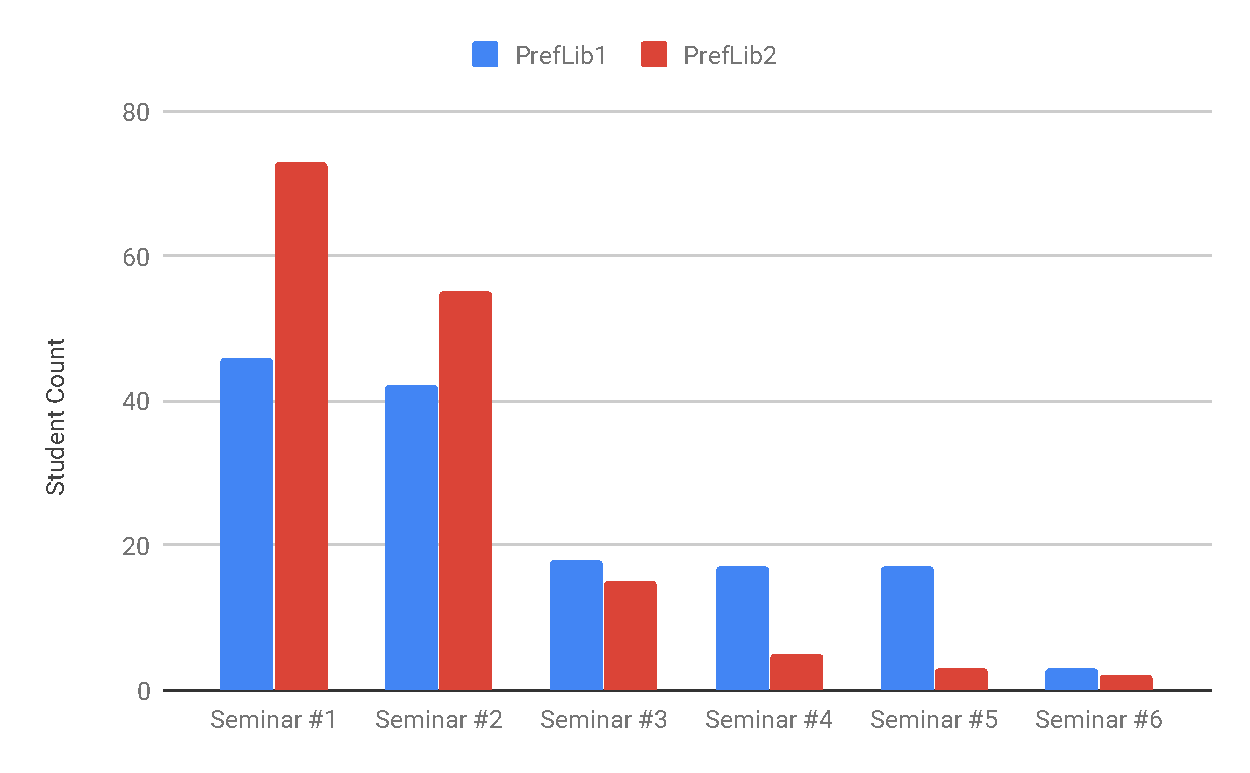
\includegraphics[width=0.8\linewidth]{assets/plots/prelib-distr.pdf}
    \caption{Preference distributions for first-ranked seminars for both PrefLib datasets}
    \label{fig:preflib-distribution}
\end{figure}

Figure \ref{fig:preflib-distribution} shows the preference distributions for the student's first choice in both datasets after removing the always first-ranked seminar. We can see that in both datasets, students clearly strongly prefer two seminars. However in the first dataset, there are 3 more seminars that are also decently popular, while in the second dataset the majority of students really prefers the two dominant seminars. Generally, those datasets indicate that the preference structure of real-world datasets is not likely to be uniformly distributed.

\subsubsection{Random Zipf-Distributed Preference Lists}
To better simulate real-world preference structures than by using a uniform distribution, a power-law distribution can be applied. According to Zipf's law the frequency of a word in a large sample, is proportional to it's position in a frequency table \cite{Zipf}. This law can also be applied for creating synthetic seminar distribution. Using this type of distribution with some additional randomization yields the following preference list structure when seminar and student counts are similar to the first PrefLib dataset:

  \begin{figure}[h!]
    \centering
    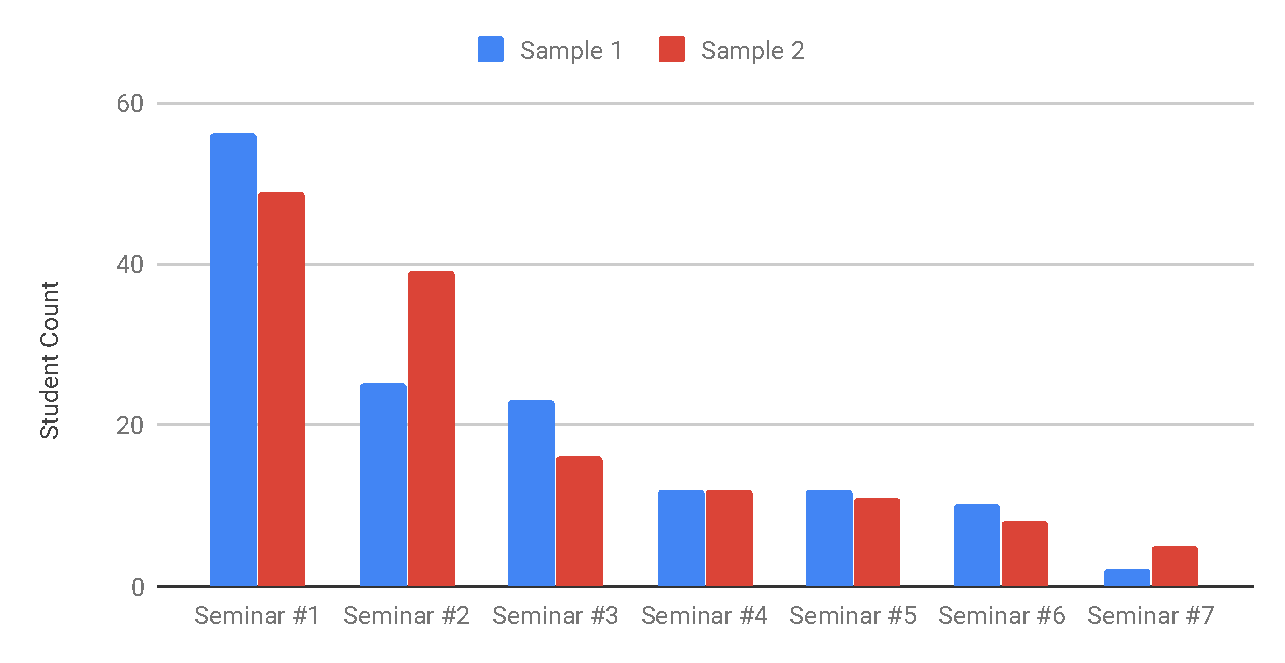
\includegraphics[width=0.8\linewidth]{assets/plots/zipfian-distr.pdf}
    \caption{Two sample Zipfian preference distribution for first-ranked seminars}
    \label{fig:zipfian-distribution}
\end{figure}

To create the dataset, for each student a seminar is randomly drawn using the Zipfian distribution and added to the his preference list until the desired preference-list length has been reached. Comparing Figure \ref{fig:zipfian-distribution} to Figure \ref{fig:preflib-distribution} shows somewhat similar results, which should make this generator relevant for the benchmark. 

\subsection{Methodology}
The goal of this experiment is quantifying some of the optimality criteria defined in Section \ref{sec:optimality} to compare the selection of algorithms empirically and find answers to the research questions proposed in Section \ref{sec:research-q}. Due to the fact that real-world data for student enrollments is not widely available, it is important to note that the results of this experiment will be biased by the selection of data available. However, by using the available real datasets and a few different synthetic datasets it should be possible to find answers to the proposed research questions and to better understand the differences of different approaches.

\subsubsection{Benchmark Setup}
The benchmark is performed by a Kotlin program that generates test data and then executes each of the algorithms with the same input. The program then collects the results and computes statistics on each matching, which are saved into a file. When using synthetic data, the program will generate between 10-50 different instances to account for the randomness. All experiments are run on a workstation with a 4-core (8 threads) Intel Core i5 8250U processor and 16GB of memory. The following types of instances will be used:
\begin{enumerate}
  \item PrefLib datasets
  \item Small Zipfian dataset ($\sim$200 students)
  \item Large Zipfian dataset ($\sim$2500 students)
  \item Large Uniform with incomplete preferences (5000 Students)
  \item Large Uniform dataset with complete preferences (5000 Students)
\end{enumerate}

\subsubsection{Metrics}
We already know that all of the algorithms under consideration produce pareto-optimal matchings, however, it will be necessary to measure popularity. If the Popular-CHA algorithm finds a matching, we know that it's the popular matching, however if the algorithm cannot find a matching it could be possible that one of the other algorithms produces such a matching. In general, given the definitions for Popularity that we have used before, it is not possible to check if a given matching is popular without comparing it to all other matchings. However this is infeasable due to the exponential runtime complexity of that comparison, which is why we will just compare the matchings produced by the five algorithms for Popularity. Given two matchings $m, m' \in \mathcal{M}$, we say that $m$ is more popular than $m'$ if the number of students prefering $m$ is greater than the number of students prefering $m'$. 
In addition to comparing Popularity, the following other metrics will be used:
\begin{itemize}
  \item \textbf{Profile}: The profile of the matching as defined in Section \ref{sec:profile} given as an array.
  \item \textbf{Average Rank \& Standard Deviation}: The average and standard deviation of the matched students' ranks. A matched student's rank corresponds to the position of his match on his preference list. In case there are unassigned students, two numbers will be given for this metric. First the metric excluding unassigned students is given and then in parentheses the metrics including unassigned students, weighted with the maximum rank is given.
  \item \textbf{Worst Rank}: In conjunction with the previous metric, we will also look at the worst rank that exists in a matching.
  \item \textbf{Unassigned-Count}: The number of unassigned students in a matching.
  \item \textbf{Runtime}: The runtime of the algorithm in milliseconds. Only the runtime of the actual algorithm in C++ is measured without parsing the input data or printing the result.
  \item \textbf{Existence}: This metric is only interesting for the Popular-CHA algorithm and will indicate if the algorithm was able to compute a matching for a given instance.
\end{itemize}

These metrics should be a sufficient selection to quantify a matching's optimality and therefore should make it possible to answer the research questions from section \ref{sec:research-q}.

\subsection{Results}

\subsubsection{PrefLib1 dataset}
The PrefLib datasets contain strict, complete preferences for a small number of students and seminars. Table \ref{tab:results-preflib1} shows results for executing the algorithms on the first dataset. Unfortunately, the Popular CHA algorithm did not compute a matching, however we can also see that the Mod-Popular algorithm computed a matching that ties in popularity with the matching produced by the Hungarian algorithm. Unsurprisingly, in terms of rank the Hungarian algorithm produces the best matching with an average rank of 1.513 and a standard deviation of 0.829.

\begin{table}[h!]
  \centering
  \resizebox{\textwidth}{!}{%
  \begin{tabular}{|l|l|l|l|l|l|}
  \hline
  Metric & RSD & Max PaCHA & Hungarian & Popular CHA & Mod-Popular \\ \hline
  Average Rank & 1.787 & 1.924 & \cellcolor[HTML]{9AFF99}1.513 & \cellcolor[HTML]{FFCCC9}n/a & 1.276 (2.342) \\ \hline
  Rank SD & 1.136 & 1.426 & \cellcolor[HTML]{9AFF99}0.829 & \cellcolor[HTML]{FFCCC9}n/a & 0.540 (3.079) \\ \hline
  Unassigned-Count & 0 & 0 & 0 & \cellcolor[HTML]{FFCCC9}146 & \cellcolor[HTML]{FFCCC9}16 \\ \hline
  Runtime & <1ms & 19ms & 13ms & 1ms & 1ms \\ \hline
  More Popular & 1.5 & 1.5 & \cellcolor[HTML]{9AFF99}3.5 & 0 & \cellcolor[HTML]{9AFF99}3.5 \\ \hline
  Worst Rank & 7 & 7 & 4 & - & 3 / Unassigned \\ \hline
  Exists & yes & yes & yes & \cellcolor[HTML]{FFCCC9}no & yes \\ \hline
  \end{tabular}%
  }
  \caption{Summary of the results for PrefLib1}
  \label{tab:results-preflib1}
\end{table}

When not taking the unassigned students into account, the Mod-Popular CHA algorithm performs even better on the rank metrics, however if taking the unassigned students into account it performs worst among all algorithms. Figure \ref{fig:preflib1-rank-distribution} shows the rank distribution for the algorithms that produced a matching and makes clear that, the Mod-Popular CHA algorithm assigns more students to their first rank at the cost of leaving a lot of students unassigned. 

\begin{figure}[h!]
  \centering
    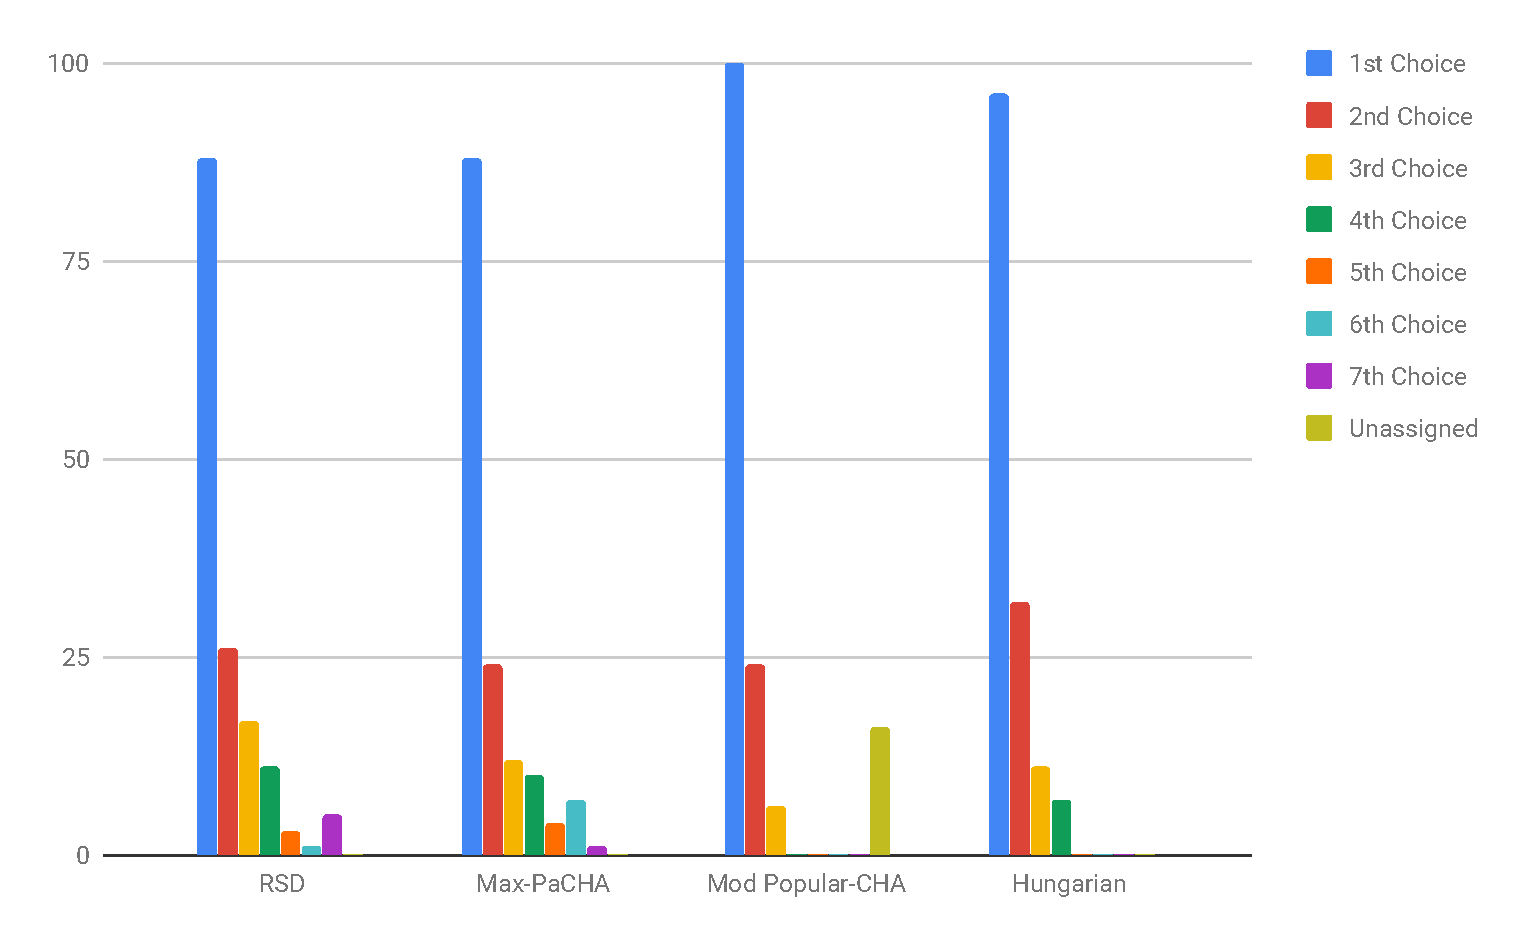
\includegraphics[width=0.9\linewidth]{assets/plots/preflib1-ranks.pdf}    
    \caption{Rank distribution for PrefLib1 Dataset. Note: Popular CHA failed.}
    \label{fig:preflib1-rank-distribution}
\end{figure}

What else is surprising with this instance is that the greedy RSD algorithm performs better than Max PaCHA in regards to the rank metric, even though both are of maximum cardinality. Surprisingly the algorithms also tie for popularity for this instance, even though RSD performs better from a rank perspective. Runtime wise, there are no surprises other than the fact that the Hungarian algorithm is faster than Max PaCHA for this instance. However, with this size of input the runtime results are not that significant.

\subsubsection{PrefLib2 dataset}
\begin{table}[h!]
  \centering
  \resizebox{\textwidth}{!}{%
  \begin{tabular}{|l|l|l|l|l|l|}
  \hline
  Metric & RSD & Max PaCHA & Hungarian & Popular CHA & Mod-Popular \\ \hline
  Average Rank & 1.712 & \cellcolor[HTML]{FFCCC9}1.758 & \cellcolor[HTML]{9AFF99}1.640 & 1.686 & 1.686 \\ \hline
  Rank SD & 0.797 & \cellcolor[HTML]{FFCCC9}0.878 & \cellcolor[HTML]{9AFF99}0.728 & 0.787 & 0.787 \\ \hline
  Unassigned-Count & 0 & 0 & 0 & 0 & 0 \\ \hline
  Runtime & <1ms & 41ms & 45ms & 9ms & 10ms \\ \hline
  More Popular & 1 & 0 & \cellcolor[HTML]{96FFFB}2 (+2 Ties) & \cellcolor[HTML]{96FFFB}2 (+2 Ties) & \cellcolor[HTML]{96FFFB}2 (+2 Ties) \\ \hline
  Worst Rank & 5 & 5 & 3 & 3 & 3 \\ \hline
  Exists & yes & yes & yes & yes & yes \\ \hline
  \end{tabular}%
  }
  \caption{Summary of the results for PrefLib2}
  \label{tab:results-preflib2}
\end{table}

Table \ref{tab:results-preflib2} shows the results for the PrefLib2 dataset. We can see that the Popular CHA algorithm finds a matching, which is why the last two columns are identical. What's interesting about the results is that the the matchings produced by the Hungarian and Popular CHA algorithm tie in popularity, even though they are different in regards to the rank metrics. 

What else stands out is that RSD again produces a better matching than Max PaCHA in regards to the rank metrics. In fact, the matching produced by the Max PaCHA algorithm performs worst in terms of rank, even though its runtime is the second highest. Overall the runtimes are still low, with all of them being lower than 50ms, which should make all algorithms usable for real world applications for similarly sized instances. However it has to be noted that the matching produced by RSD gets close in terms of rank to the matching produced by the Hungarian algorithm, even though the it is about 50 times faster.

\begin{figure}[h!]
  \centering
    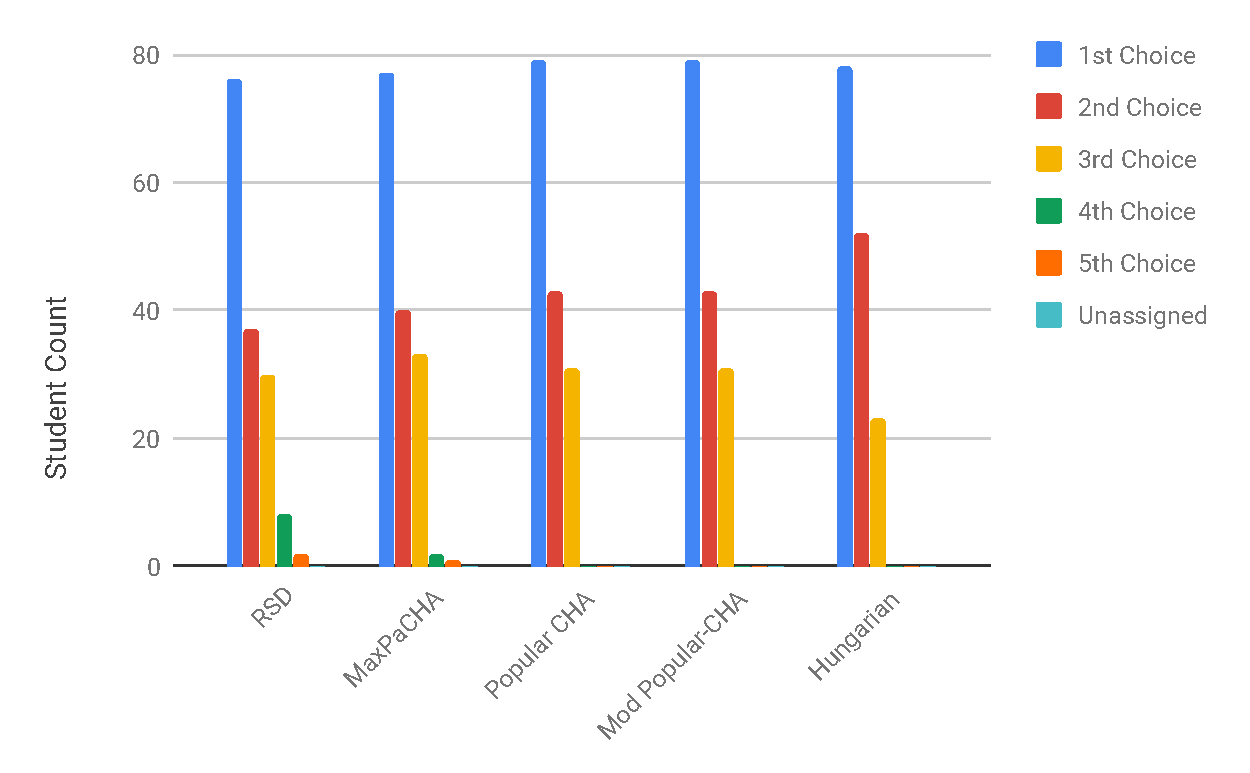
\includegraphics[width=0.9\linewidth]{assets/plots/preflib2-ranks.pdf}    
    \caption{Rank distribution for PrefLib2 Dataset.}
    \label{fig:preflib2-rank-distribution}
\end{figure}

Figure \ref{fig:preflib2-rank-distribution} shows the preference distribution of all five algorithms. We can see that RSD and Max-PaCHA assign some students to their 4th or 5th choice, which explains why they perform worse in terms of rank. Unsurprisingly the matching produced by the Hungarian algorithm has the best rank-profile.

\subsubsection{Small Zipfian datasets}

\begin{table}[h!]
  \centering
  \resizebox{\textwidth}{!}{%
  \begin{tabular}{|l|l|l|l|l|l|}
  \hline
  Metric & RSD & Max PaCHA & Hungarian & Popular CHA & Mod-Popular \\ \hline
  Average Rank & 1.893 (2.014) & 1.910 & \cellcolor[HTML]{9AFF99}1.481 & 1.646 & 1.523 (1.913) \\ \hline
  Rank SD & 1.451 (1.782) & 1.457 & \cellcolor[HTML]{9AFF99}0.716 & 1.034 & 0.874 (2.121) \\ \hline
  Unassigned-Count & 2 & 0 & 0 & 0 & \cellcolor[HTML]{FFCCC9}7 \\ \hline
  Runtime & \textless{}1ms & 54ms & 60ms & 7ms & 10ms \\ \hline
  More Popular & 1 & 1.65 & 3.05 & 0.7 & \cellcolor[HTML]{9AFF99}3.6 \\ \hline
  Worst Rank & \cellcolor[HTML]{FFCCC9}8 & \cellcolor[HTML]{FFCCC9}8 & \cellcolor[HTML]{9AFF99}5 & \cellcolor[HTML]{9AFF99}5 & 6 \\ \hline
  Exists & yes & yes & yes & \cellcolor[HTML]{FFCCC9}4/50 exist & yes \\ \hline
  \end{tabular}%
  }
  \caption{Average results for small Zipfian dataset with 50 runs}
  \label{tab:results-zipfian-small}
\end{table}

Since the Zipfian datasets have a somewhat similar preference distribution as the PrefLib datasets we should see similar results, however parameters can be tuned such as preference list length and student count. We will begin by looking at a similarly sized dataset as the Preflib datasets and then begin deviating the student \& seminar count. Table \ref{tab:results-zipfian-small}
shows the average results for 50 test runs using the Zipfian Dataset with 10 seminars and about 200 students. Out of the 50 instances, the Popular CHA algorithm only found a matching for four instances. When it found a matching, it did so quite fast and the matching was on average better rank-wise than all other algorithms except for the Hungarian algorithm. In terms of popularity, the Mod-Popular CHA algorithm actually outperformed all algorithms (equal to Popular-CHA if the matching exists) for most instances, even though rank-wise it does not perform as well as the Hungarian algorithm. However, the Hungarian algorithm produced more popular matchings than most other algorithms, and for some instances even more popular than the Mod-Popular CHA algorithm.

\subsubsection{Large Zipfian datasets}
Using a large dataset with a Zipfian distribution yields similar results. Table \ref{tab:results-zipfian-medium} summarizes the average results for 10 test runs with datasets that contain about 2500 students and 35 seminars.

\begin{table}[h!]
  \centering
  \resizebox{\textwidth}{!}{%
  \begin{tabular}{|l|l|l|l|l|l|}
  \hline
  Metric & RSD & Max PaCHA & Hungarian & Popular CHA & Mod-Popular \\ \hline
  Average Rank & 1.911 (5.287) & \cellcolor[HTML]{FFCCC9}2.109 & \cellcolor[HTML]{9AFF99}1.824 & - & 1.694 (4.746) \\ \hline
  Rank SD & 1.225 (10.41) & \cellcolor[HTML]{FFCCC9}1.383 & \cellcolor[HTML]{9AFF99}1.029 & - & 1.087 (9.967) \\ \hline
  Unassigned & \cellcolor[HTML]{FFCCC9}10\% & \cellcolor[HTML]{9AFF99}0\% & \cellcolor[HTML]{9AFF99}0\% & 100\% & \cellcolor[HTML]{FFCCC9}8.6\% \\ \hline
  Runtime & \cellcolor[HTML]{9AFF99}3ms & 2190ms & \cellcolor[HTML]{FFCCC9}65730ms & - & \cellcolor[HTML]{9AFF99}168ms \\ \hline
  More Popular & 1.1 & 1.65 & 3 & 0 & \cellcolor[HTML]{9AFF99}4 \\ \hline
  Worst Rank & 7 & 7 & \cellcolor[HTML]{9AFF99}6 & - & 7 \\ \hline
  Exists & yes & yes & yes & \cellcolor[HTML]{FFCCC9}0/10 & yes \\ \hline
  \end{tabular}%
  }
  \caption{Average results for large Zipfian dataset (2500 Students) with 10 runs}
  \label{tab:results-zipfian-medium}
\end{table}

Again, the Popular CHA algorithm was not very successful and found no matching in any of the test runs. However, the Mod-Popular CHA algorithm always produced more popular matchings than all of the other algorithms, even though 8.6\% of the students were left unassigned on average. When taking the unassigned students out of the rank metrics, the Mod-Popular CHA algorithm produces matchings with the best average rank and standard deviation, while having the second lowest runtime. In contrast to that, the Hungarian algorithm always assigned all students, however needed on average 65 seconds to do so. This confirms the theoretical observations about runtime and shows that using the Hungarian algorithm is potentially not feasible for large instances.

\begin{figure}[h!]
  \centering
    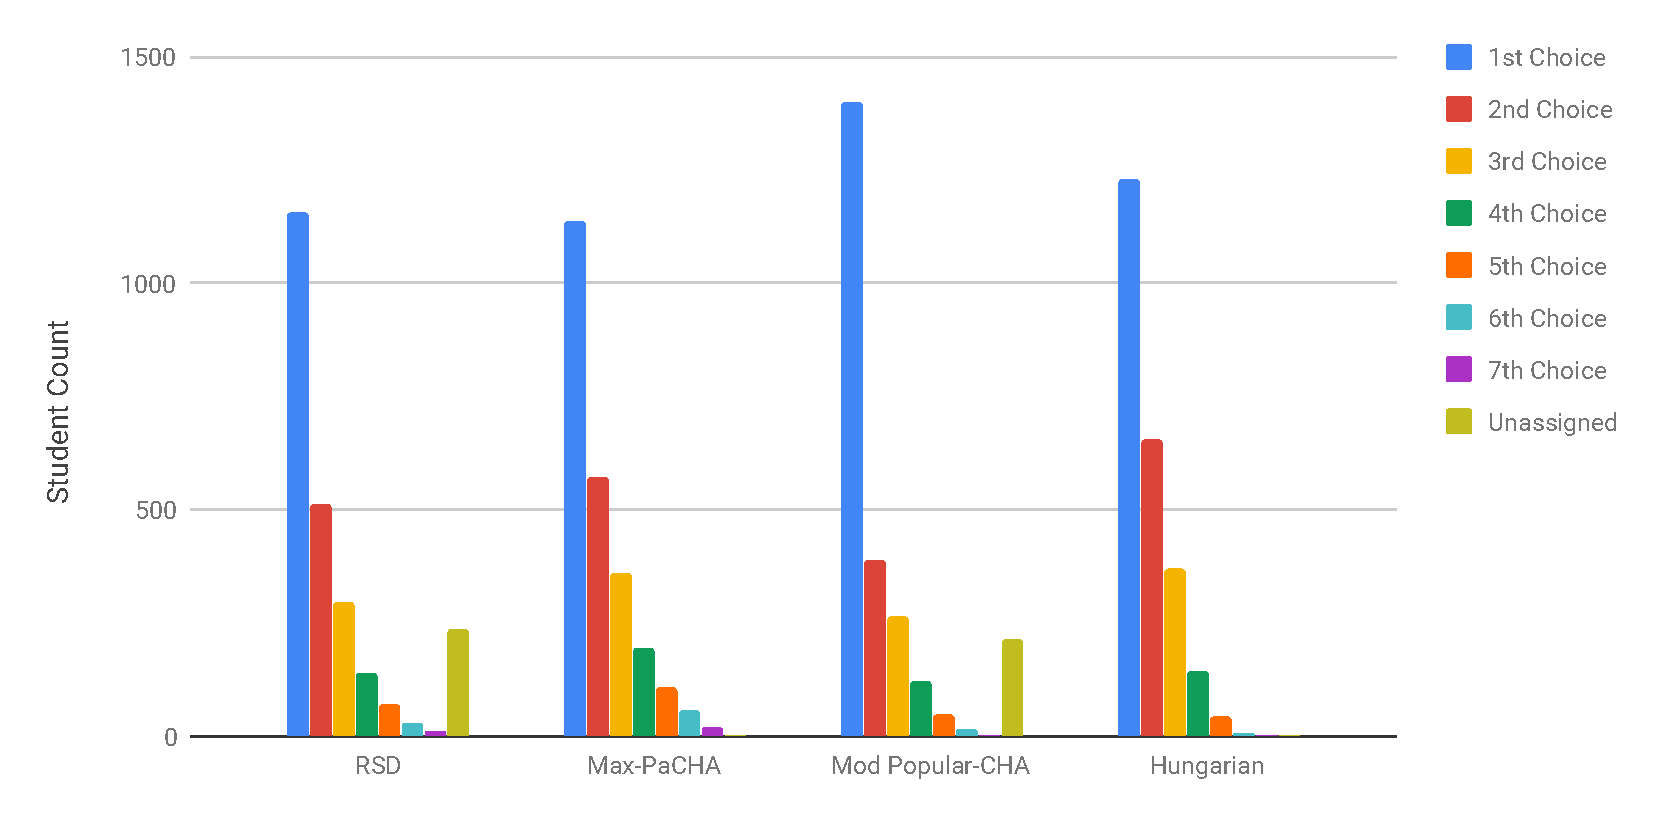
\includegraphics[width=0.9\linewidth]{assets/plots/zipfian-medium.pdf}
    \caption{Rank distribution for large Zipfian dataset.}
    \label{fig:zipfian-medium-distribution}
\end{figure}

Figure \ref{fig:zipfian-medium-distribution} shows the rank distributions for all algorithms but Popular CHA. We can see that Mod Popular-CHA is able to outperform the other algorithms in terms of popularity by maximizing the number of students being assigned to their first choice. However, the Hungarian algorithm produced more balanced matchings, where the most students were assigned to their top three choices, while also leaving no student unassigned.

\subsubsection{Large uniform dataset with incomplete preferences}
This large uniform dataset contains 50 seminars and 5000 students, who each randomly picked 10 seminars with equal probability.  

\begin{table}[h!]
  \centering
  \resizebox{\textwidth}{!}{%
  \begin{tabular}{|l|l|l|l|l|l|}
  \hline
  Metric & RSD & Max PaCHA & Hungarian & Popular CHA & Mod-Popular \\ \hline
  Average Rank & 1.119 (1.265) & \cellcolor[HTML]{FFCCC9}1.133 & \cellcolor[HTML]{9AFF99}1.041 & 1.093 & 1.083 \\ \hline
  Rank SD & 0.647 (2.778) & \cellcolor[HTML]{FFCCC9}0.713 & \cellcolor[HTML]{9AFF99}0.2 & 0.508 & 0.486 \\ \hline
  Unassigned & 0.28\% & 0\% & 0\% & 0\% (90\%) & 0\% \\ \hline
  Runtime & 13ms & 6175ms & \cellcolor[HTML]{FFCCC9}55815ms & 257ms & 221ms \\ \hline
  More Popular & 1.65 & 1.15 & \cellcolor[HTML]{9AFF99}3.45 & 0.3 & \cellcolor[HTML]{9AFF99}3.45 \\ \hline
  Worst Rank & 10 & 10 & \cellcolor[HTML]{9AFF99}2 & 8 & 10 \\ \hline
  Exists & yes & yes & yes & 1/10 & yes \\ \hline
  \end{tabular}%
  }
  \caption{Average results for large uniform dataset with incomplete preferences.}
  \label{tab:results-uniform-large}
\end{table}

Table \ref{tab:results-uniform-large} shows the average results when executing each algorithm 10 times. Unfortunately the Popular CHA algorithm only found a matching for one out of the 10 instances, but when it did, it performed quite well in terms of rank. However, the Mod-Popular CHA algorithm was on average able to find better matchings in less time than the Popular CHA mechanism. What also stands out is that Mod-Popular CHA and the Hungarian algorithm are tied for popularity in every instance, but runtime wise Mod-Popular CHA performs far better than the Hungarian algorithm. What needs to be noted though, is that the Hunarian algorithm outperforms all other algorithms in terms of profile by having the worst rank in all matchings be 2. All algorithms assign more than 94\% of the students to their first choice, but the Hungarian algorithm only assigns students to their first or second choice.  

\subsubsection{Large uniform dataset with complete preferences}
When using the same size dataset as before, but with complete preference lists, the results show some interesting insights. Table \ref{tab:results-uniform-large-complete} shows that Popular-CHA found a matching for every instance, which helps answer the question if preference list length has an effect on Popular CHA. For this dataset, Popular CHA and the Hungarian algorithm always produce matchings of the same popularity, which means that there exists more than one popular matching for every instance. 

\begin{table}[h!]
  \centering
  \resizebox{\textwidth}{!}{%
  \begin{tabular}{|l|l|l|l|l|l|}
  \hline
  Metric & RSD & Max PaCHA & Hungarian & Popular CHA & Mod-Popular \\ \hline
  Average Rank & \cellcolor[HTML]{FFCCC9}1.198 & 1.190 & \cellcolor[HTML]{9AFF99}1.039 & \cellcolor[HTML]{9AFF99}1.076 & \cellcolor[HTML]{9AFF99}1.076 \\ \hline
  Rank SD & \cellcolor[HTML]{FFCCC9}1.543 & 1.469 & \cellcolor[HTML]{9AFF99}0.193 & \cellcolor[HTML]{9AFF99}0.453 & \cellcolor[HTML]{9AFF99}0.453 \\ \hline
  Unassigned & 0\% & 0\% & 0\% & 0\% & 0\% \\ \hline
  Runtime & 11ms & 7922ms & \cellcolor[HTML]{FFCCC9}57141ms & 228ms & 219ms \\ \hline
  More Popular & 0.5 & 0.5 & \cellcolor[HTML]{9AFF99}3 & \cellcolor[HTML]{9AFF99}3 & \cellcolor[HTML]{9AFF99}3 \\ \hline
  Worst Rank & \cellcolor[HTML]{FFCCC9}30 & \cellcolor[HTML]{FFCCC9}27 & \cellcolor[HTML]{9AFF99}2 & 9 & 9 \\ \hline
  Exists & yes & yes & yes & \cellcolor[HTML]{9AFF99}10/10 & yes \\ \hline
  \end{tabular}%
  }
  \caption{Average results for large uniform dataset with complete preferences.}
  \label{tab:results-uniform-large-complete}
\end{table}

Another things that stands out is the fact that RSD and Max PaCHA produce matchings with high worst-ranks of 30 and 27 respectively. Overall these two algorithms perform worse or equal on all metrics than Popular CHA and the Hungarian algorithm, which makes them less appealing for this kind of dataset. Given the low average runtime of 219ms the Mod-Popular CHA algorithm seems to be a good option when the size of the instance is too large for the Hungarian, while still performing well on the rank-related metrics. Even though Popular-CHA and the Hungarian algorithm tie in popularity, it should be assumed that a matching with a worst rank of 2 is more popular among the students than a matching of worst rank 9. 

\subsection{Conclusion}
The experiments have revealed some interesting insights that should help answering the research questions from section \ref{sec:research-q}.

\begin{enumerate}
  \item \textbf{Effect of different preference distributions:} Unsurprisingly, the algorithms performed better on the rank metrics, when the preferences were distributed uniformly. In fact, the Hungarian algorithm was able to assign on average more than 94\% (Table \ref{tab:results-uniform-large-complete}) of the students to their first choice when the preference distribution was uniform.
  \item \textbf{Failure rate of Popular-CHA:} The experiments have shown that \mbox{Popular-CHA} fails to find a matching quite often, especially if the preference lists are short and not uniformly distributed. When using the Zipfian datasets (Tables \ref{tab:results-zipfian-medium}, \ref{tab:results-zipfian-small}), Popular-CHA only found a matching for 4/60 instances. Even for uniform distributions and incomplete preference lists (table \ref{tab:results-uniform-large}) the algorithm only found a matching for 1/10 instances. Making the preference lists complete makes it easier for the algorithm to find matchings as shown in Table \ref{tab:results-uniform-large-complete}.
  \item \textbf{Performance of Mod-Popular-CHA:} The modified version of Popular-CHA was able to find comparatively good matchings in a short amount of time, while also usually producing more or equally popular matchings as the other algorithms. For many instances Mod-Popular-CHA tied the Hungarian algorithm for popularity and was able to produce good matchings in terms of the rank metrics in a fraction of the time.
  \item \textbf{Cost of giving up on strategy-proofness:} Surprisingly RSD produced on average better matchings on most metrics than Max-PaCHA, while also being by far the fastest algorithm. However, RSD usually produced the highest percentage of unassigned students, but the modified Popular-CHA algorithm usually outperformed RSD on most metrics, while also having a relatively low runtime. In the real-world datasets (PrefLib), RSD left no students unassigned and got close to the Hungarian algorithm in terms of rank, but also had 7 as the worst rank, compared to 4 for the Hungarian algorithm. 
  \item \textbf{Popularity as a meaningful metric:} For many instances we could not find the one popular matching, as Popular-CHA simply failed, but when it didn't, the worst rank, average rank and rank standard deviation was higher than what the Hungarian algorithm produced. Another interesting insight was that matchings produced by Mod-Popular-CHA usually tied in popularity with those produced by the Hungarian algorithm, even though Mod-Popular-CHA often left a few students unassigned. For instance in Figure \ref{fig:zipfian-medium-distribution}, Mod-Popular-CHA left on average 8.6\% of the students unassigned but the matchings were still classified as more popular or just as popular as the matchings produced by the Hungarian algorithm. This shows that a popular matching can maximize the number of students ranked to their first choice at the cost of some students being matched to a low-ranking seminar or even none. This makes it questionable, whether popularity is a meaningful optimality criteria for the student and seminar usecase, as it should be a goal to assign as many students as possible and to make all students equally satisfied with their match instead of finding the biggest possible subset of students, where everyone is satisfied.
  \item \textbf{The effect of short preference lists:} The experiments have shown that short preference lists make it more likely for Popular-CHA to not find a matching, as well as making it more likely for RSD to produce matchings with more unassigned students.
\end{enumerate}

In summary, the matchings produced by the Hungarian algorithm usually perform best in all of the metrics, except for runtime where it performs the worst by far. However, for the student-seminar use case that should not be a problem, because most instances will be smaller than what we have tested with. In fact, when using the real world datasets (see Table \ref{tab:results-preflib1} and \ref{tab:results-preflib2}), the runtime differences for the different mechanisms were insignifcant. For large instances, the modified Popular-CHA algorithm performed well and it could still be optimized even further for matching more students. The algorithm as it was in described in section \ref{impl:mod-max-pop}, does not try to assign students that were left unmatched by the Hopcroft-Karp algorithm, which could easily be done by either using a simple mechanism like RSD or even using the Hungarian algorithm on the set of unassigned students. Neither modification guarantees that the final matching would be popular or of maximum cardinality, but it could improve the matching. Therefore it would make the Mod-Popular-CHA algorithm a fast heuristic that should, according to the experiments, perform better than RSD and Max-PaCHA for most instances, while still keeping the runtime low.

\newpage
\section{Extensions to the problem}
For the bulk of this thesis, we have looked at many-to-one matching problems with one-sided preferences, as this settings makes the most sense for the student-seminar application. However, there is a wide range of similar problems and extensions that are also worth mentioning. This section will present some of those problems and key results from the literature. 

\subsection{Two-Sided preferences}


\subsection{Many-to-Many matchings}

\subsection{Online variant}
When solving the online-variant of the problem, the whole input is not available from the start. That means that the input needs to be processed piece by piece, or more formally: Given a bipartite weighted graph $(U, V, E)$, where $U$ is known to the algorithm, vertices in $V$ are unknown, but arrive one at a time, while also revealing their incident edges, find a matching that maximizes some objective function. These algorithms could be of interest in the case of a first-come first-serve course allocation system, or in other areas such as DVD-rental or online-advertisement allocation systems.\cite{Mehta:Online}

In the case of student-seminar assignments, we would assume that the set of courses and their capacities is known beforehand, and the students arrive later. One of the algorithms we have seen in section \ref{chapter:algorithms} can be used for this problem, namely the RSD-algorithm. As a matter of fact, the algorithm will produce the same results for the offline and online case, given that the order in which students are processed is identical.

\subsubsection{Online max-cardinality matching}
There has been lots of research in particular on finding maximum-cardinality matchings with online inputs. The online-inputs are classified by how much information the algorithm possesses about the input order. For now, we will only consider the \textbf{Adversarial order}, where we assume no knowledge of the query sequence, which means that only $U$ is known at the beginning of the algorithm, while we have no knowledge of $V$ and $E$ or the order they appear in.\cite{Mehta:Online} To measure performance we will use the \textbf{competetive ratio} of an algorithm which is defined as follows. Given an instance of the problem $I$, the value of the objective function for the online algorithm is given as $ALG(I)$, and the value of the objective function for the best offline algorithm is given as $OPT(I)$. The competetive ratio is now computed as follows: $C.R.=\frac{ALG(I)}{OPT(I)}$.\cite{Mehta:Online}

Simple algorithms for this online problem, are a greedy algorithm, that matches arriving vertices to any available neighbor, or a random approach that matches arriving vertices to a random neighbor. These mechanisms achieve a competetive ratio of $\frac{1}{2}$.\cite{Mehta:Online} An optimal, but yet simple algorithm was introduced by Karp et al.\cite{Karp:Online}, which achieves a competetive ratio of $1 - \frac{1}{e} \simeq 0.63$. The algorithm, called Ranking, begins by permutating the known vertices of $U$ in a random permutation $\pi$, i.e. we assign a random priority number to each $u \in U$. Each incoming vertex $v \in V$ is then assigned to an available neighbor, with the smallest value of $\pi(u)$. In detail the algorithm looks like this:

\begin{algorithm} % enter the algorithm environment
    \caption{Ranking} 
    \label{alg:ranking} % and a label for \ref{} commands later in the document
    \begin{algorithmic} % enter the algorithmic environment
        \State \textbf{Offline:} Pick a random, uniform permutation $\pi$ of U
        \ForEach {arriving vertex $v \in V $}
            \If{$v$ has no available neighbors}
                \State continue
            \EndIf
            \State Match $v$ to the neighbor $u \in U$ with the smallest value $\pi(u)$
        \EndFor
    \end{algorithmic}
\end{algorithm}

\newpage
\section{Discussion}

The goal of this chapter is to provide an overview of both the theoretical and practical results and to give detailed comparisons and a trade-off analysis of the algorithms.

\subsection{Discussion of Theoretical and Practical Results}
Drawing back to the theoretical results from Table \ref{tab:algorithm-comparison}, we have already seen that none of the algorithms produce matchings will all of the desired criteria. In particular, strategy-proofness cannot be achieved if trying to maximize a matching's cardinality. Popular-CHA, which theoretically is strategy-proof, unfortunately does not always find a matching, which makes it less suitable for real-world applications. Both the results from Diebold et al. (Section \ref{sec:practical-results-lit}) and our experiment show that Popular-CHA fails for about 90\% of the tested instances. There is also no known algorithm that efficiently computes the popular matching if it is not of maximum cardinality, which makes it questionable as to whether or not popularity should be considered when designing such a matching system. The results from Table \ref{tab:results-preflib2} and \ref{tab:results-uniform-large-complete} show that the matchings produced by Popular-CHA and the Hungarian algorithm often tie in terms of popularity, even though the Hungarian algorithm clearly performs better on other metrics. Looking at the rank distributions of some matchings in Figure \ref{fig:preflib2-rank-distribution} and \ref{fig:zipfian-distribution}, we have seen that (Mod-) Popular-CHA attempts to maximize the number of students assigned to their first choice in order to find a popular matching. It is highly questionable if this property is desirable over having a matching with a lower rank average and especially a lower rank standard deviation, which is what the Hungarian algorithm typically finds. For this reason, we would argue that popularity as an optimality criteria should not be of high importance when selecting a matching mechanism for the CHA problem. The results have shown that popular matchings, compared to profile-based optimal matchings, do not explicitly attempt to provide a good match for every student, but instead give some students a bad or no match in order to give the majority of students a better match.

Another surprising finding from our experiments is that Max-PaCHA usually performs worse than all other algorithms on the rank metrics, including RSD. This can easily be explained by the fact that Max-PaCHA essentially performs a local search from an initial (maximum-cardinality) matching and terminates when finding one and only one local optima. Contrary to that, the greedy approach (RSD) also performs a local search; however, achieves better average ranks due to the fact that it does not attempt to maximize the matching's cardinality. Comparing RSD and Max-PaCHA to the other algorithms, the Hungarian algorithm and Mod-Popular-CHA should be preferred due to the fact that they simply performed better on almost all other metrics in the experiments. However, if using a strategy-proof mechanism is a requirement, RSD should obviously be used.

\subsection{Potential Algorithmic Improvements}\label{sec:improvements}
In Section \ref{impl:mod-max-pop}, we briefly discussed a modified version of the Popular-CHA algorithm that was used in the experiment to gain insights on failing instances of Popular-CHA. However, the modified algorithm leaves some room for optimization, as it does not attempt to match students that were either unmatched or assigned to their last-resort preference after performing the maximum cardinality matching. A simple way of improving this algorithm is to use one of the other algorithms (e.g. RSD) on that unmatched subset of students. Doing this would not worsen the matching's popularity, because being matched to any seminar is better than not being matched at all from a popularity perspective. Using this modified mechanism could be a good alternative to using the Hungarian algorithm when using large instances where runtime could be a problem. 

Besides that, different algorithmic approaches could be used for computing a profile-based optimal matching. In Section \ref{algo:assignment}, we presented the approach of reducing the matching problem to the assignment problem or by using flow-networks to find a rank-maximal matching. For the use case of student and seminar matchings, it can be assumed that instances will be relatively small; however, the experiments have also shown that the Hungarian algorithm's runtime is quite poor compared to the other algorithms when using larger instances. For instance, when using about 5000 students (Table \ref{tab:results-uniform-large} and \ref{tab:results-uniform-large-complete}),
the Hungarian algorithm took, on average, about 60 seconds to find a matching, compared to about 230ms for the Popular-CHA mechanism. A faster algorithm for finding a profile-based optimal matching, Rank-Max, is presented by Sng et al. \cite{SngThesis}. They show that for a given instance $I$ of the CHAT (with ties) problem, the algorithm finds a rank-maximal matching in $\mathcal{O}(\min(z^*\sqrt{C}, C + z^*)m)$, where $z^*$ is the maximal rank of an edge in an optimal solution of $I$, $C$ is the total capacity of the houses in $I$ and $m$ is the sum of the lengths of all preference lists in $I$. Compared to that, the version of the Hungarian algorithm used for the experiments has a runtime of $\mathcal{O}((C+n_1)^3)$ with $n_1$ being the number of students and $C$ again being the total capacity of all seminars. While the theoretical runtime of Rank-Max is much better than of the Hungarian algorithm, we have seen that for small, real-world instances like the PrefLib datasets (Table \ref{tab:results-preflib1}), the runtime of the Hungarian algorithm was still below 20ms.

\subsection{System Design Recommendations}
As alluded to in the previous two subsections, the Hungarian algorithm provides the best results and, from a distribution perspective, probably the fairest distribution out of all algorithms. Important properties of the algorithm are that it finds matchings of maximal cardinality, as well as matchings with the lowest average rank combined with a low rank standard deviation. While the runtime of that algorithm was the highest among all other algorithms presented, performance should not be a problem for real-world student-seminar matching scenarios, where the instances are somewhat small. To improve performance, the Max-Rank algorithm \cite{SngThesis} could be used for finding an exact result or, for very large instances, the Mod-Popular-CHA algorithm can be used. To improve the performance of all algorithms, it would also help to require students to supply at least $k$ preferences, where $k$ could be a fixed fraction of the total seminar count. The experiments have indicated that longer preference lists, especially when power-law-like preference distributions are used, make the algorithms perform better.

Besides that, the online variant of the problem can be solved using a first-come first-serve mechanism like RSD or an algorithm like Ranking (Algorithm \ref{alg:ranking}) that maximizes cardinality in the online scenario (See Appendix \ref{sec:online-variants} for more information on the online problem).

\newpage
\section{Conclusion}

The goal of this thesis has been to present and analyze different matching mechanisms and their properties for one-to-many matching scenarios with one-sided preferences. A variety of optimality criteria exist, but in the end, it is evident that, none of the algorithms presented produce matchings that fulfill all of the optimality criteria. 

The experiments conducted have shown that the resulting matchings vary quite a lot by algorithm and structure of the instance. In summary, the Hungarian algorithm usually outperformed all other algorithms on most metrics; but, it also had by far the highest runtime. To improve the runtime, different algorithms can be used, such as Rank-Max, that also compute profile-based matchings in almost linear time. Another insight from the experiments was that Popular-CHA failed to find matchings for a majority of the instances; however, we discussed a simple modified version of the algorithm that usually produced better results than RSD and Max-PaCHA, while having a much lower runtime than the Hungarian algorithm. Still, according to the results from the experiment, popularity seemed to be a less desirable criteria, due to the fact that popular matchings often only optimize the match for a subset of the students, while leaving the other students with a bad or no match. Therefore, we can recommend the Hungarian or Rank-Max algorithm for the use case of student-seminar matching. To improve the resulting matchings and make strategic manipulation harder, a matching system could require students to supply at least $k$ preferences. This would also partially eliminate the Hungarian's algorithm biggest disadvantage, which was that students are encouraged to provide short preference lists.

As part of this thesis, we have also presented an interactive web-system that allows university administrations to manage and solve such matching problems. The system relies on the C++ algorithms that were used for the benchmark and should offer good performance for typical instances.  

\newpage
\pagenumbering{Roman}

\bibliography{main}
\bibliographystyle{ieeetr}

% Erzeugen der Selbständigkeitserklärung auf einem neuen Blatt:
\selbstaendigkeitserklaerung{\today}

\end{document}
